\documentclass[draft]{agujournal2019}
\usepackage{amsmath}
\usepackage{url} 
\usepackage{lineno}
\usepackage[inline]{trackchanges} % track changes. 
\usepackage{soul}
\linenumbers

\draftfalse

\journalname{JGR: Earth Surface}

\begin{document}

\title{Linking landslide patterns to landscape evolution in the northern Colombian Andes}

\authors{Edier Aristizábal\affil{1,2}, Oliver Korup\affil{2,3}}

\affiliation{1}{Departamento de Geociencias y Medio Ambiente, Universidad Nacional de Colombia, Medellín, Colombia}
\affiliation{2}{Institute of Environmental Science and Geography, University of Potsdam, Germany}
\affiliation{3}{Institute of Geosciences, University of Potsdam, Germany}

\correspondingauthor{Edier Aristizábal}{evaristizabalg@unal.edu.co}

\begin{keypoints}
\item This study sheds light on the relationship between landscape evolution and landslide spatial distribution in the Colombian Andes.
\item Tectonic uplift, base-level fall, catchment rejuvenation and drainage reorganization influence the distribution of landslides.
\end{keypoints}

\begin{abstract}
Landslides are among the most recognisable processes and landforms of erosion in tectonically active mountains. Yet, how the distribution of landslides relates to topographic metrics of landscape evolution remains partly unresolved. We examine various morphometric attributes (hypsometric integral, local slope, elevation, local relief, lineaments, river longitudinal profiles, knickpoints, $\chi$ coordinate and local channel steepness) that characterise the interaction between hillslopes and channels to explain the distribution of both modern and prehistoric landslides in the northern Colombian Andes. We find strong links between the clustered occurrence of these landslides and high rates of tectonic uplift. We propose a conceptual model to explain how tectonic uplift, base-level changes and landscape rejuvenation might influence landslide occurrence. We argue that drainage reorganization and knickpoint migration drives by tectonic uplift might play a crucial role in determining the observed landslide distribution. We infer that long-term landscape evolution may condition actual landslide occurrence in the northern Colombian Andes.
\end{abstract}

%%%%%%%%%%%%%%%%%%%%%%%%%%%%%%%%%%%%%%%%%%%%%%%%%%%%%%
\section{Introduction}
\par Modern views of landscape evolution emphasize the dynamic interaction between tectonic activity and climatically modulated shifts of mass across the land surface \cite{Davies2021, Whittaker2012, Irasema2002}. These perturbations may cause transient states, but landscapes inherently move toward an equilibrium where rock uplift and denudation are balanced  \cite{Whittaker2012, Wobus2006, Whipple2004}. River networks are primary conveyors by which perturbations propagate through the landscape, thus forcing the surrounding hillslopes to evolve in response to changes in base level \cite{Whipple2004, howard1994}. Consequently, the geometric configuration of rivers and hillslopes encodes valuable information about tectonic and climatic disturbances \cite{whipple2017, stock1999}, offering insights into the dominant geomorphic processes, which in active mountain belts often involve abundant landsliding \cite{Larsen2012, korup2010, Montgomery2002, Campforts2020, Broeckx2020}.

\par  Yet, the controls of landslide spatial patterns remain poorly understood beyond the scope of individual triggers such as earthquakes or rainstorms \cite{yanites2018}. For example, susceptibility studies attempt to explain landslide distribution in space, but concentrate on the hillslope scale and use local parameters as terrain indices, slope material properties, or land-cover attributes as statistical predictors \cite{reichenbach2018, soeters1996, montgomery1994}. Yet, how these possible controls play out in terms of entire landslide patterns instead of local (or pixel-wise) susceptibility remains uncertain and thus often described as stochastic \cite{Benda1997}. 

\par Another view is that landslides form as a local hillslope response to upstream knickpoint migration in response to base-level fall into catchments in disequilibrium \cite{Wobus2006, hovius2006, Whipple2002}. Thus, the dynamics of the channel network control landslide distribution  \cite{montgomery1994, burbank1996}, and this response has also been observed in laboratory experiments \cite{Bigi2006, hasbargen2000}. For example, \citeA{burbank1996} used the distributions of hillslope inclinations, cosmogenic exposure and radiometric cooling ages to argue that landsliding the northwestern Himalayas is the main mechanism through which hillslopes adjust to high rates of river incision. \citeA{Larsen2012} supported this notion by reporting a significant correlation between landslide frequency, exhumation rates, and stream power in the eastern Himalayas. In a flume laboratory, \citeA{Bigi2006} examined the relationship between hillslope failure and migrating channel knickpoints, and reported a statistically significant correlation between the positions of knickpoints and the location of landslides downstream. \citeA{tsou2017} used river and hillslope morphometry to show that transient hillslopes resulting by successive rejuvenated river incisions control the distribution of deep-seated landslides and long-term slope stability in southwestern Japan. \citeA{Gallen2011} noted a similar pattern in the southern Appalachians, where local relief was higher, hillslopes steeper and landslides more abundant in tributary catchments downstream of major knickpoints. \citeA{Gallen2011} used hypsometric analyses to propose a model for determining different evolutionary stages of landscape development. This model posits that the hypsometric distribution of a catchment in equilibrium tends to be skewed toward lower elevations. When a perturbation occurs, it creates a distinct peak in the hypsometric distribution that migrates to higher elevations, moving farther away from a state of equilibrium. 

\par Landscape evolution models built on stream-power models incorporate hillslope-channel coupling and landsliding via mechanistic threshold criteria. Several authors emphasize the role of landslide controlling landscape response to catchment perturbations. For example, \citeA{Egholm2013} numerically simulated a reciprocal relationship between channel incision and landslides. The model showed positive feedback when landslides increased sediment input and accelerated fluvial incision, whereas a negative feedback emerged where excess sediment protected the river bed from erosion. \citeA{roering2015} showed how changes in rock uplift and incision alter the frequency and pattern of active landslides in the northern California Coastal Ranges. The authors proposed areas with greater uplift rates have larger, faster, and more frequent landslides. Another landscape evolution model by \citeA{Campforts2020, Campforts2022} incorporated stochastic landsliding and its effect on fluvial sediment dynamics and showed that, as rock-uplift rates increased, so did the frequency and magnitude of landslides, whereas drainage density and stream concavity decreased.

\par Considering landslides are the major natural hazard in Colombia \cite{gomez2023spatial, aristizabal2020}
and there have been no studies on the legacy of landscape evolution in landslide occurrences in the Colombian Andes, we examine whether the pattern of both recent and pre-historic landslides is linked to metrics of landscape evolution in this tectonically active area. In particular, we test the model proposed by \citeA{Gallen2011}. To this end, we check whether and how well we can objectively derive from digital topographic data different stages of landscape evolution and channel-hillslope coupling, and how these help to explain the distribution of observed landslides.

%%%%%%%%%%%%%%%%%%%%%%%%%%%%%%%%%%%%%%%%%%%%%%%%%%%%%%%%%%%%%
\section{Study area}
\par The Colombian Andes have unique geomorphic and hydroclimatological characteristics that result from their tectonic and equatorial setting. In the northern Andes, geological features are controlled by the diagonal convergence of the Nazca and Caribbean oceanic plates with the South American continental plate \cite{Cediel2003, acosta2007, trenkamp2002}. This transpressional accretion features two distinct crustal blocks: the Northern Andean Block (NAB) is moving in a north-westward direction, whereas the Panamá-Chocó Block (PCB) is moving in a south-eastward direction, in relation to the South American Plate \cite{kellogg1995}. The accretion of the PCB caused the Nazca Plate to rupture at approximately 5°N, causing flat slab subduction in the north \cite{Taboada2000}. In contrast, the south has a steeper subduction angle and active volcanoes \cite{perez2021, restrepo2019, farris2011, Taboada2000, mann1990} (Fig.~\ref{fig:geologia}A). 

\par Our study area is located north of 5°N of the Colombian Andes and encompasses mountainous terrains of the Western Cordillera (WC) and relic high-elevation (~2500 m), low-relief, and flat-toped erosional surfaces of the Central Cordillera (CC), known as the Antioqueño Plateau (AP).  Those cordilleras are separated by the Cauca canyon (Fig. \ref{fig:geologia}A). The AP is deeply incised by the main tributary of the Cauca river, the Nechi river. The WC and CC are bounded by broad and flat alluvial terrains to the west of the Atrato River, to the east by the Magdalena River, and to the north by the Cauca River. 

\par The study area covers some 48.000~ km$^2$, which we divided into 650 catchments based on catchment area and stream order. About 75\% of these drain less than 100~km$^{2}$, with median area of 36~km$^{2}$. The catchments have average slopes between 15° and 25° with difference between its highest and lowest elevations of 180~m to 380~m, which is highest at 750~m in the northern Cauca canyon (Fig.~\ref{fig:rainfall}). Narrow valleys bounded by steep slopes characterized the WC and eastern flank of the CC. 

\par The geology is composed of allochthonous terrains that have been attached to South America since the Cretaceous period \cite{Cediel2003}. The eastern terrains of Cauca-Romeral Fault System (CRFS) have intrusive Mesozoic rocks on a Precambrian basement of continental rocks and Cenozoic volcanic activity \cite{Cediel2003}, while the western terrains are made up of collided oceanic blocks and (ultra-)mafic island arcs that formed in the Late Cretaceous \cite{cardona2012arc}.

\par The PCB collides with the NAB at 15-18 mm/yr at present, producing rapid deformation in the northern Colombian Andes \cite{kellogg2019} and the reactivation of tectonic structures into oblique left-lateral normal faults and right-lateral faults \cite{acosta2007}. For the study area, \citeA{perez2021, perez2022} proposed that the collision of the PCB and slab flattening in the northernmost part of the Nazca subduction zone resulted in increased surface uplift that is highest in the western and central parts of the northern CC, but markedly lower in the east. \citeA{restrepo2019} and \citeA{Noriega2020} inferred pulses of exhumation during the Paleocene–Eocene and Oligocene–Miocene, at rates of 0.2–0.9 km/Ma, separated by phases of low exhumation rates ($<$0.02 km/Ma), that may have favoured the development of the AP. Exhumation rates were 1–1.5 mm/yr since 3~Ma for the Eastern Cordillera \cite{mora2010}. For the CC, \citeA{arboleda2015} reported rates of 1.5 km/Ma between 11 and 6 Ma, while \citeA{ott2023} proposed that Late Miocene slab flattening accelerated surface uplift ($\sim$2 km) in the northern Colombian Andes, maintaining landscape disequilibrium to the present day.

\par Generally north trending geological structures dominate the northern Colombian Andes (Fig. \ref{fig:geologia}B), especially the left-lateral Cauca-Romeral Fault System (CRFS) that separates oceanic rocks to the west from continental rocks to the east \cite{Egholm2013, ego1995}. The Itsmina Deformation Zone (IDZ), The Espíritu Santo Fault (ESF), and Palestina Fault System (PFS) are major NE-trending fault systems. The PFS is a right-lateral strike-slip structure with NW-SE antithetic faults in the intrusive rock of the CC \cite{acosta2007, feininger1970}. The ESF is a right-lateral oblique strike-slip fault with normal components in the northeast and reverse components in the southwest \cite{Noriega2020, page1986}. The IDZ marks the southern border of the PCB, and is characterized by transpressive right-lateral faults \cite{acosta2007, Taboada2000}. Lastly, the Uramita Fault system (UFS) and Arma Fault (AF) are among the NW-trending faults. While the AF is oblique normal, left-lateral, the UFS is a N-NW striking conjugate structure marking the eastern boundary of the PCB with transpressive left-lateral motion \cite{acosta2007, Taboada2000}.

\begin{figure}[ht!]
  \begin{minipage}{.48\linewidth}
    \centering
      {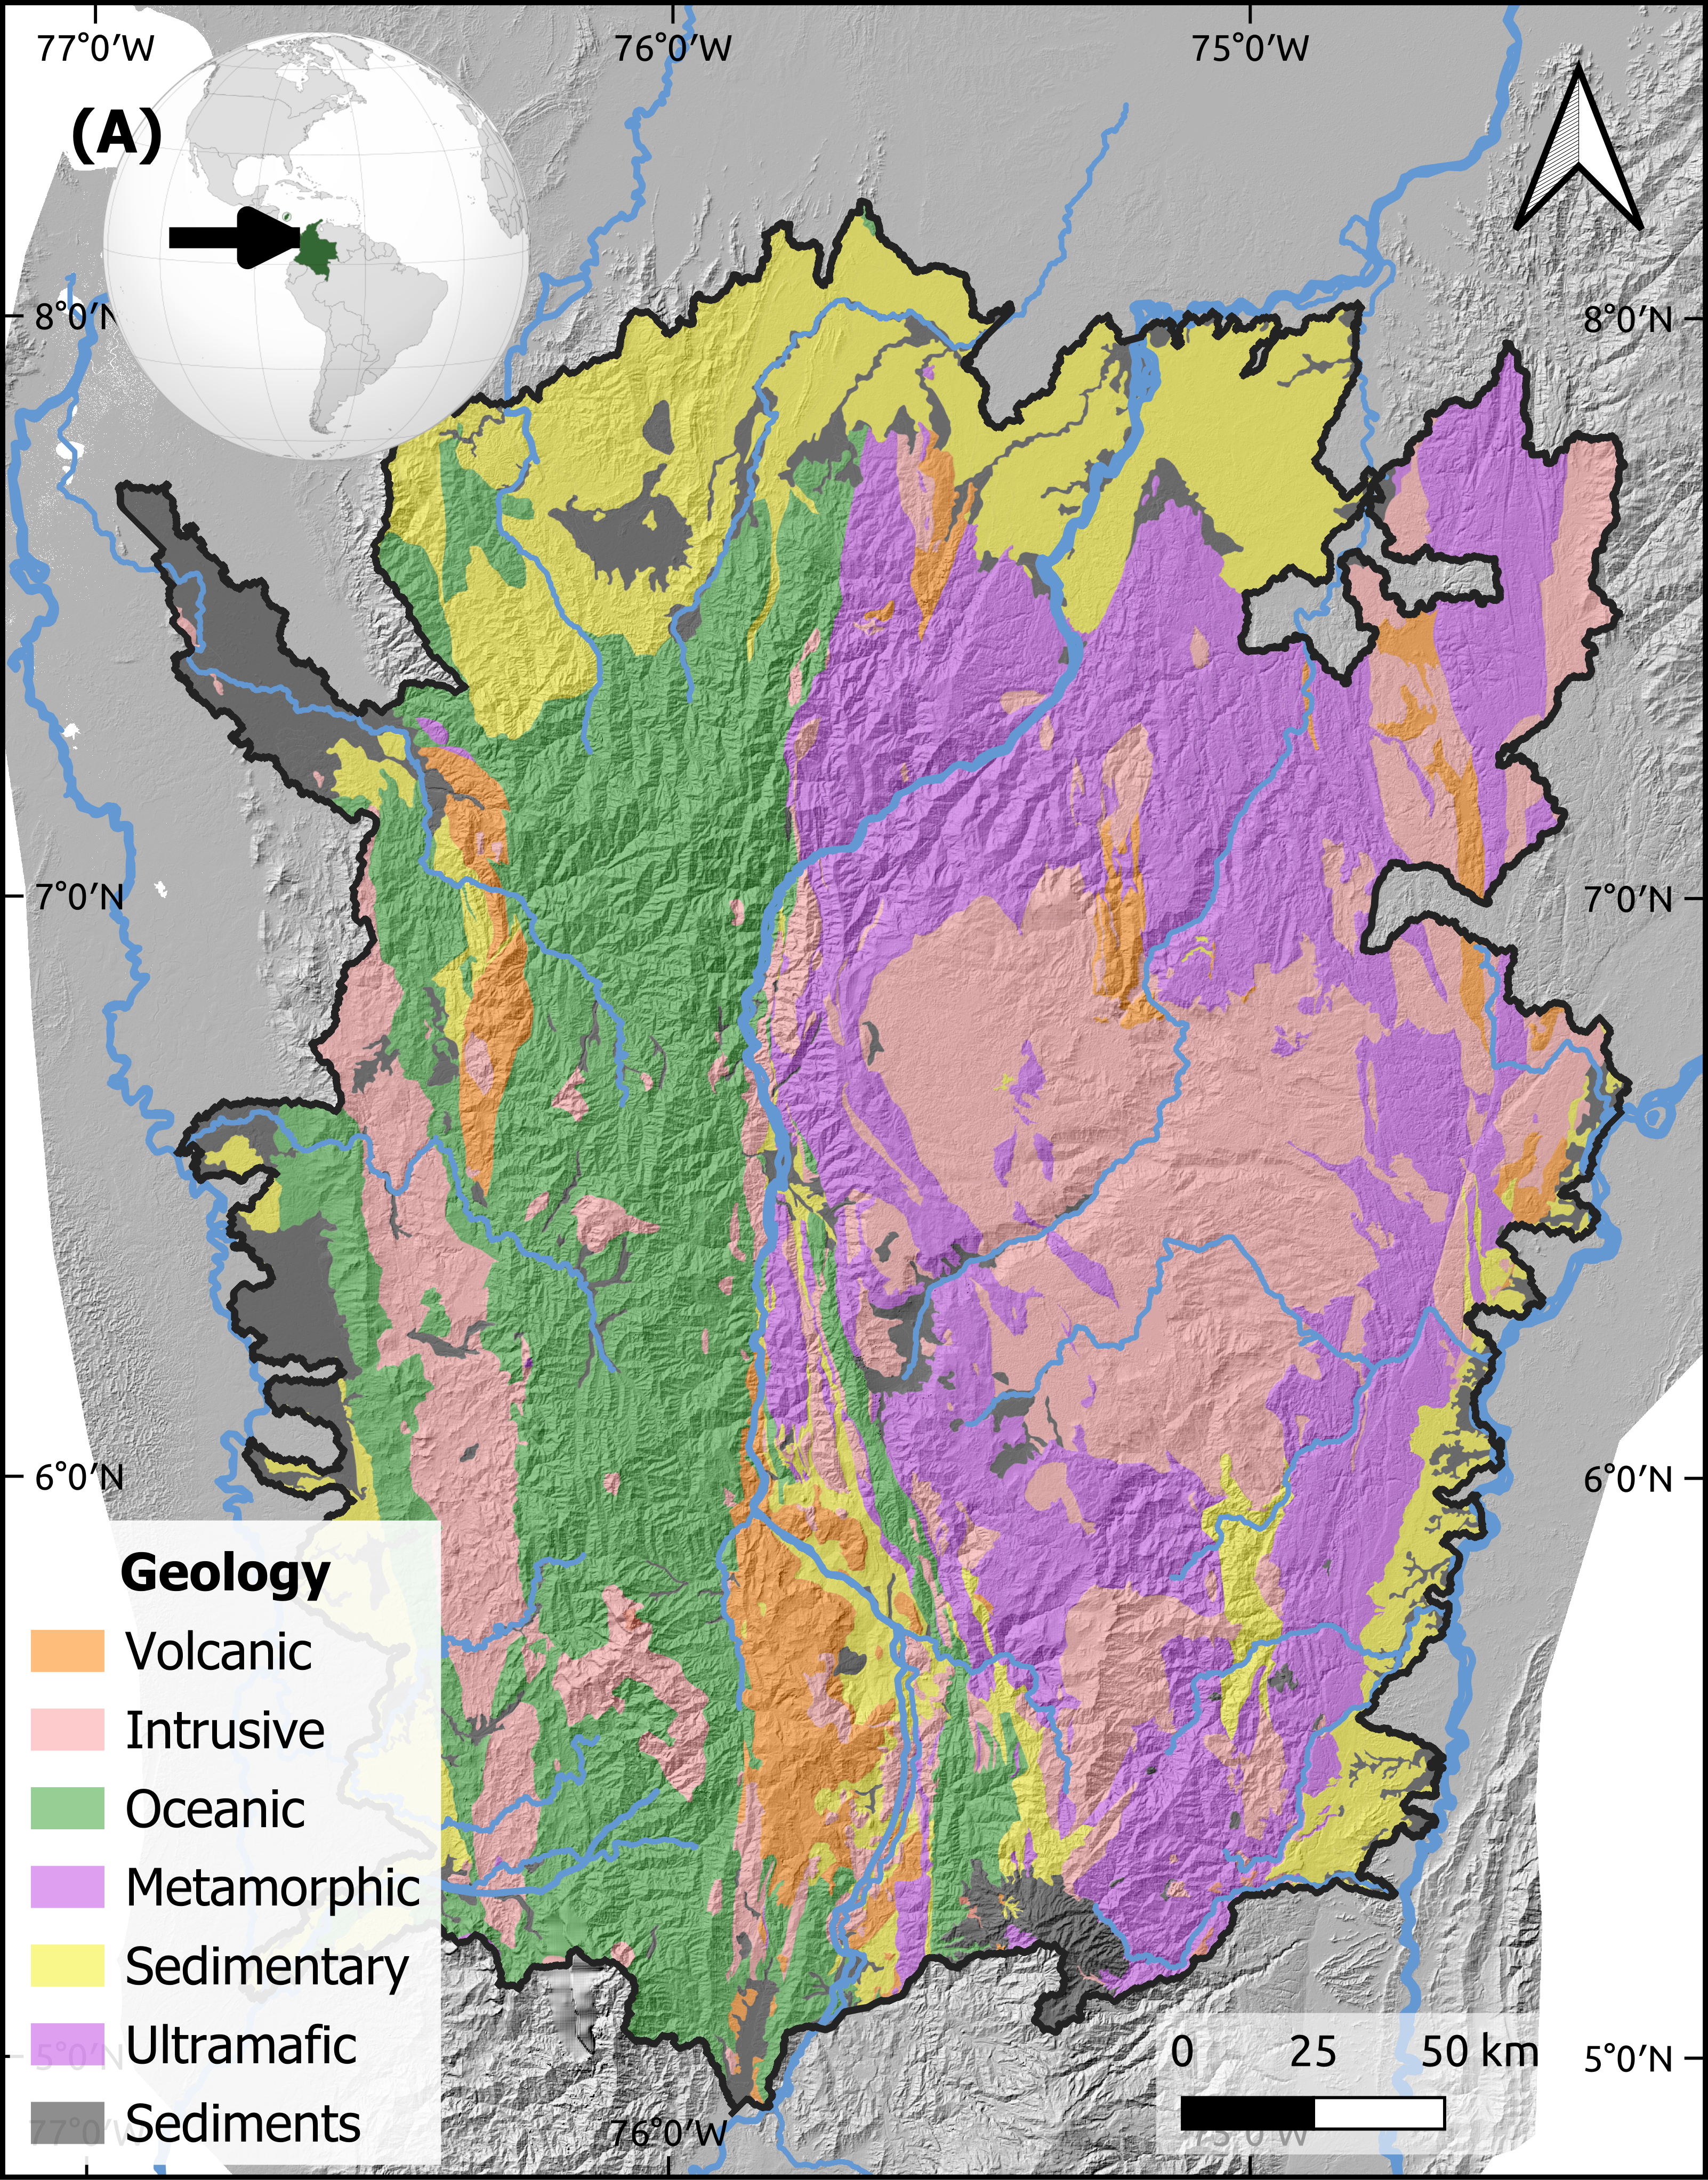
\includegraphics[width=1\textwidth]{geologia_location.png}}
  \end{minipage}\quad
  \begin{minipage}{.48\linewidth}
    \centering
      {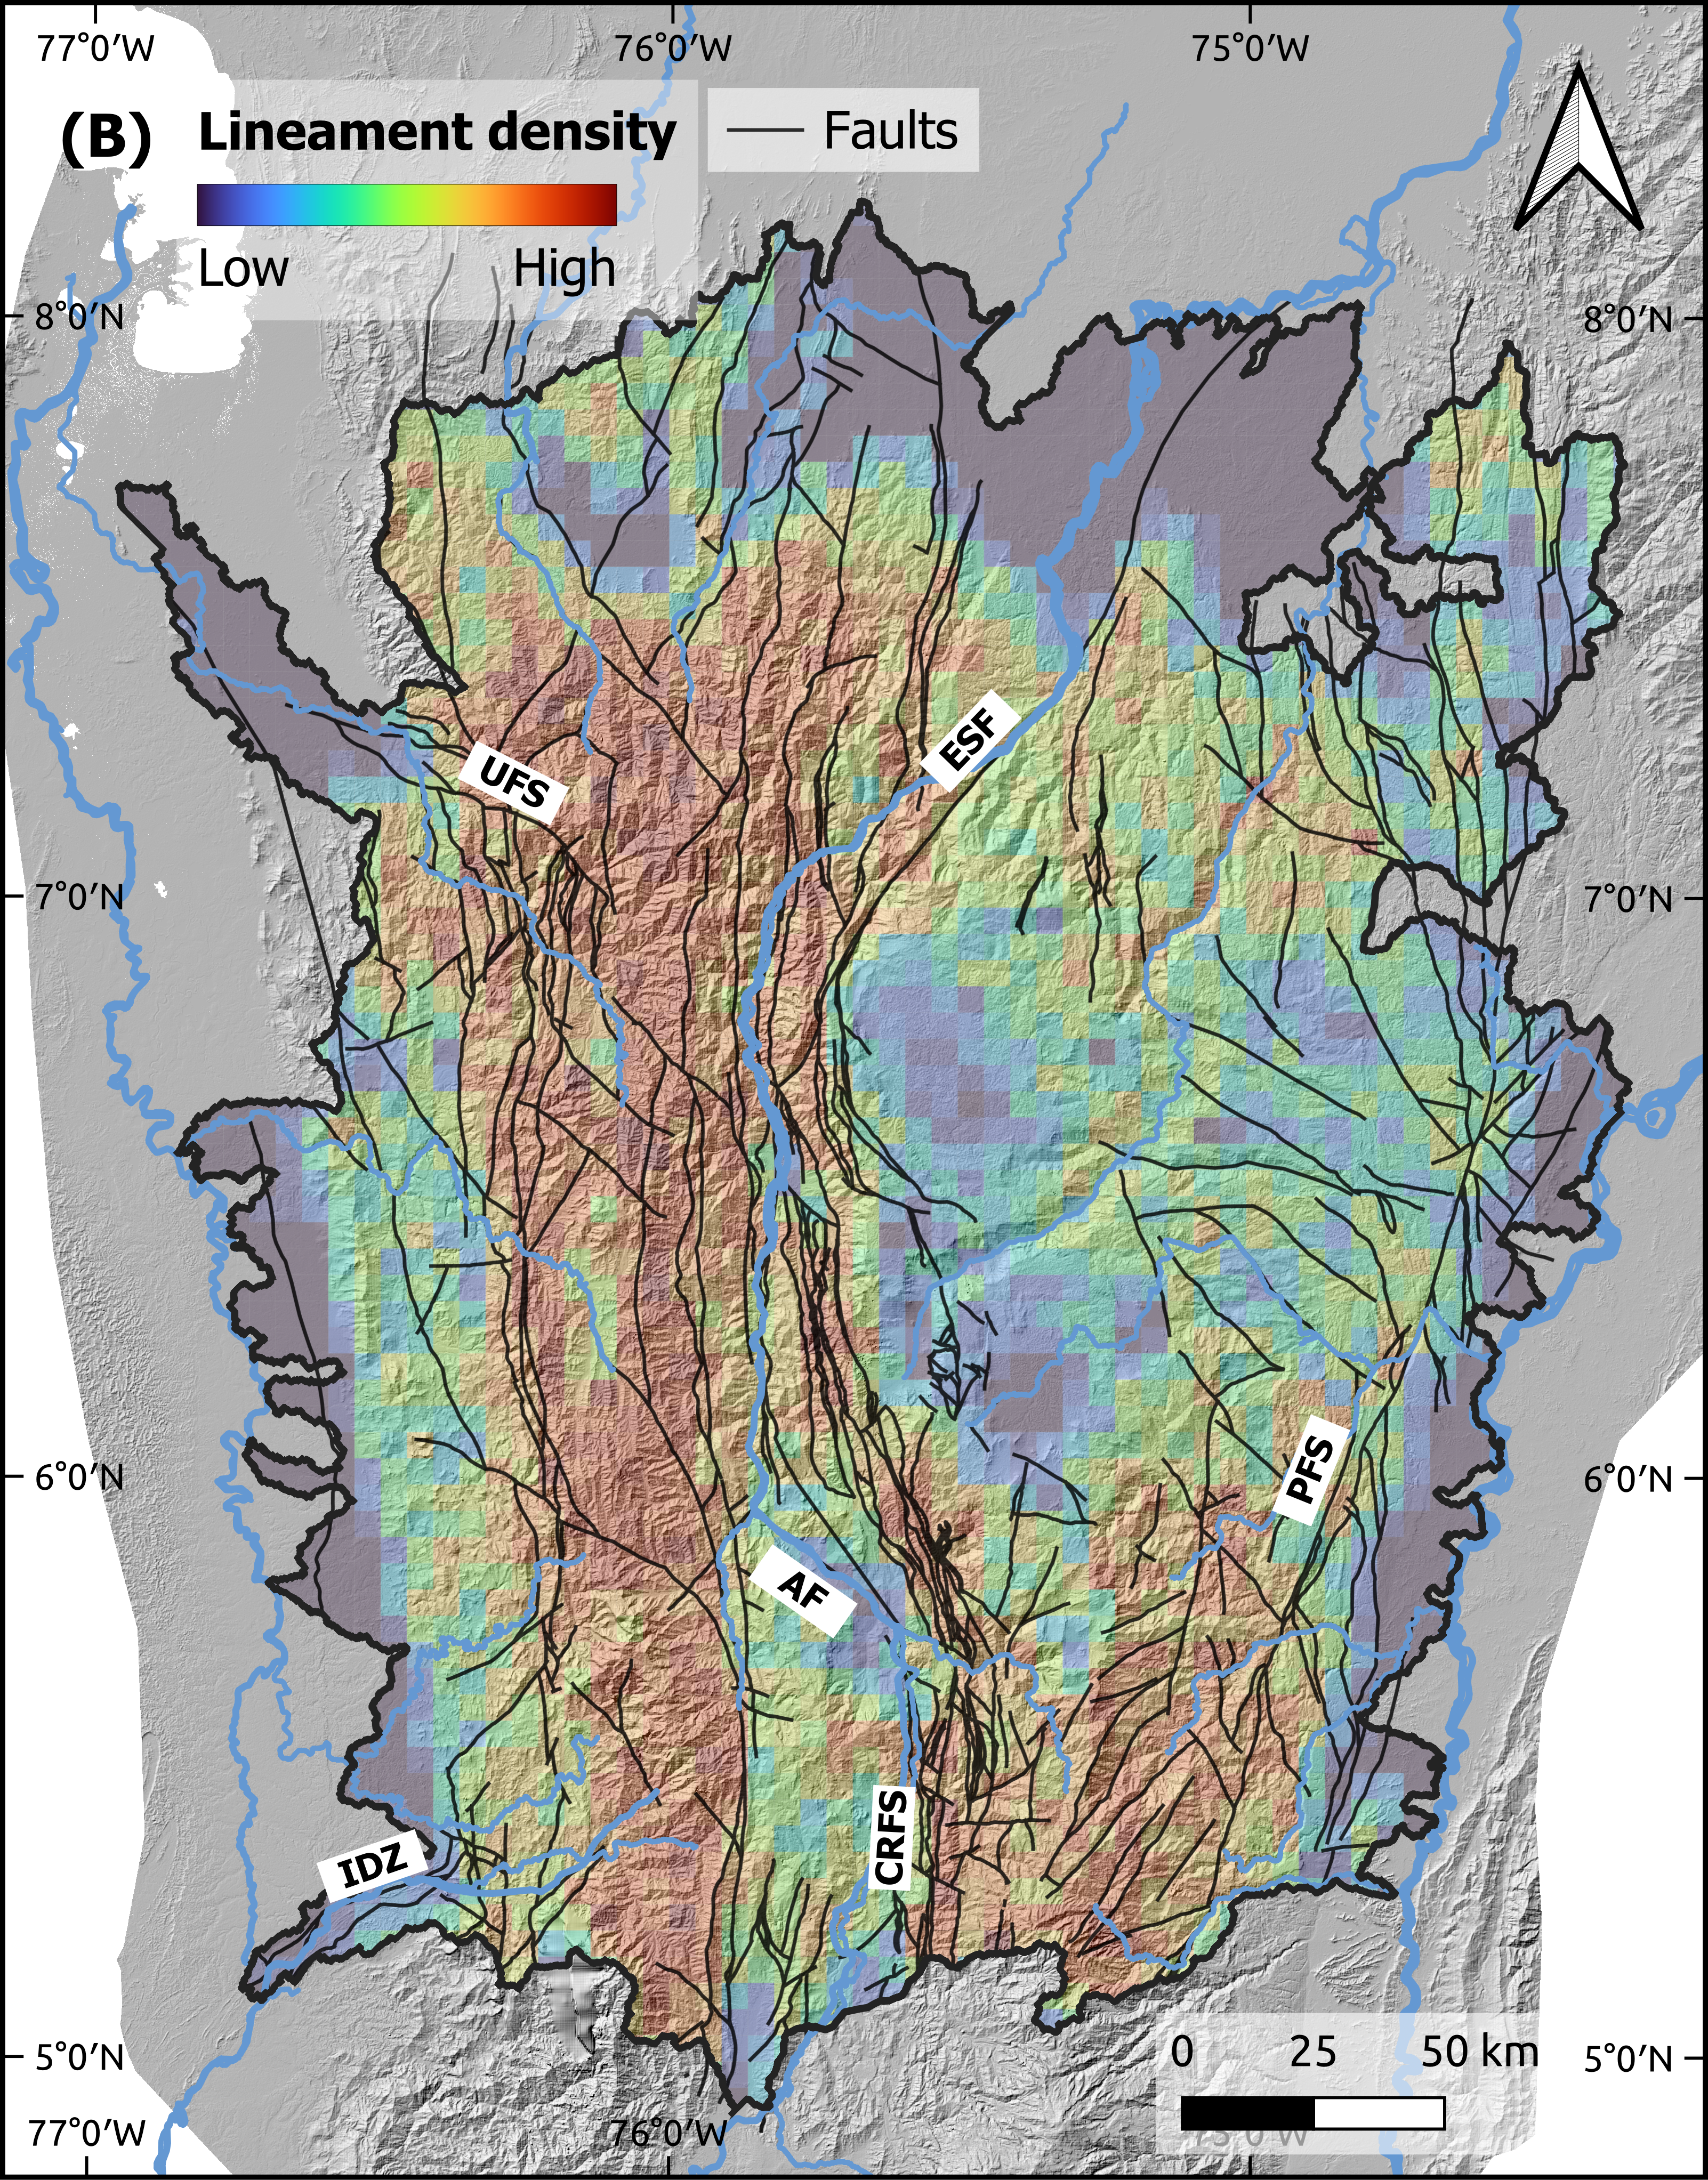
\includegraphics[width=1\textwidth]{faults.png}}
  \end{minipage}
    \caption{(A) Simplified geological map of the study area (modified from \citeA{gomez2015explanatory}). (B) Density of geological lineaments $>$1~km, estimated from eight hillshade directions with 45°-bins of azimuth at a sun elevation of 45°. Black lines are major active faults: Uramita Fault System (UFS), Espiritu Santo Fault (ESF), Arma Fault (AF), Cauca-Romeral Fault System (CRFS), Palestina Fault System (PFS), Itsmina Deformation Zone (IDZ).}
    \label{fig:geologia}
\end{figure}

\par High-relief landscape of the WC and low-relief of the CC are covered by a thick weathering profile formed by saprolitic and residual soils. On the granitoids, weathering profiles consist of deep yellowish-red (10YR 7/4) residual soils and saprolites over 50 m thick overlying up to 100 m of weathered and disintegrated rock \cite{aristizabal2005tropical}. The weathering profiles developed on the ultra-basic and metamorphic rocks are thinner. They are generally reddish orange (7.5 YR 7/6), and contain highly weathered rock fragments \cite{aristizabal2005tropical}.

\par Precipitation in the Colombian Andes has a bimodal annual cycle driven by the passage of the intertropical convergence zone (ITCZ) \cite{bedoya2019}. This seasonal pattern is modulated by the topographic gradients of the Andes that favour deep convection and trigger local intensive storms \cite{Poveda2011}. The mean annual precipitation ranges from 1,000-8,000~mm, but the distribution of rainfall is asymmetric: the more humid western range front receive more extreme amounts of between 10,000-13,000~mm \cite{poveda2000existence}, while the Cauca canyon in the center of our study area canyon contrast receives about 1,000~mm (Fig.~\ref{fig:rainfall}). 

\begin{figure}[ht!]
   \begin{minipage}{.48\linewidth}
    \centering
      {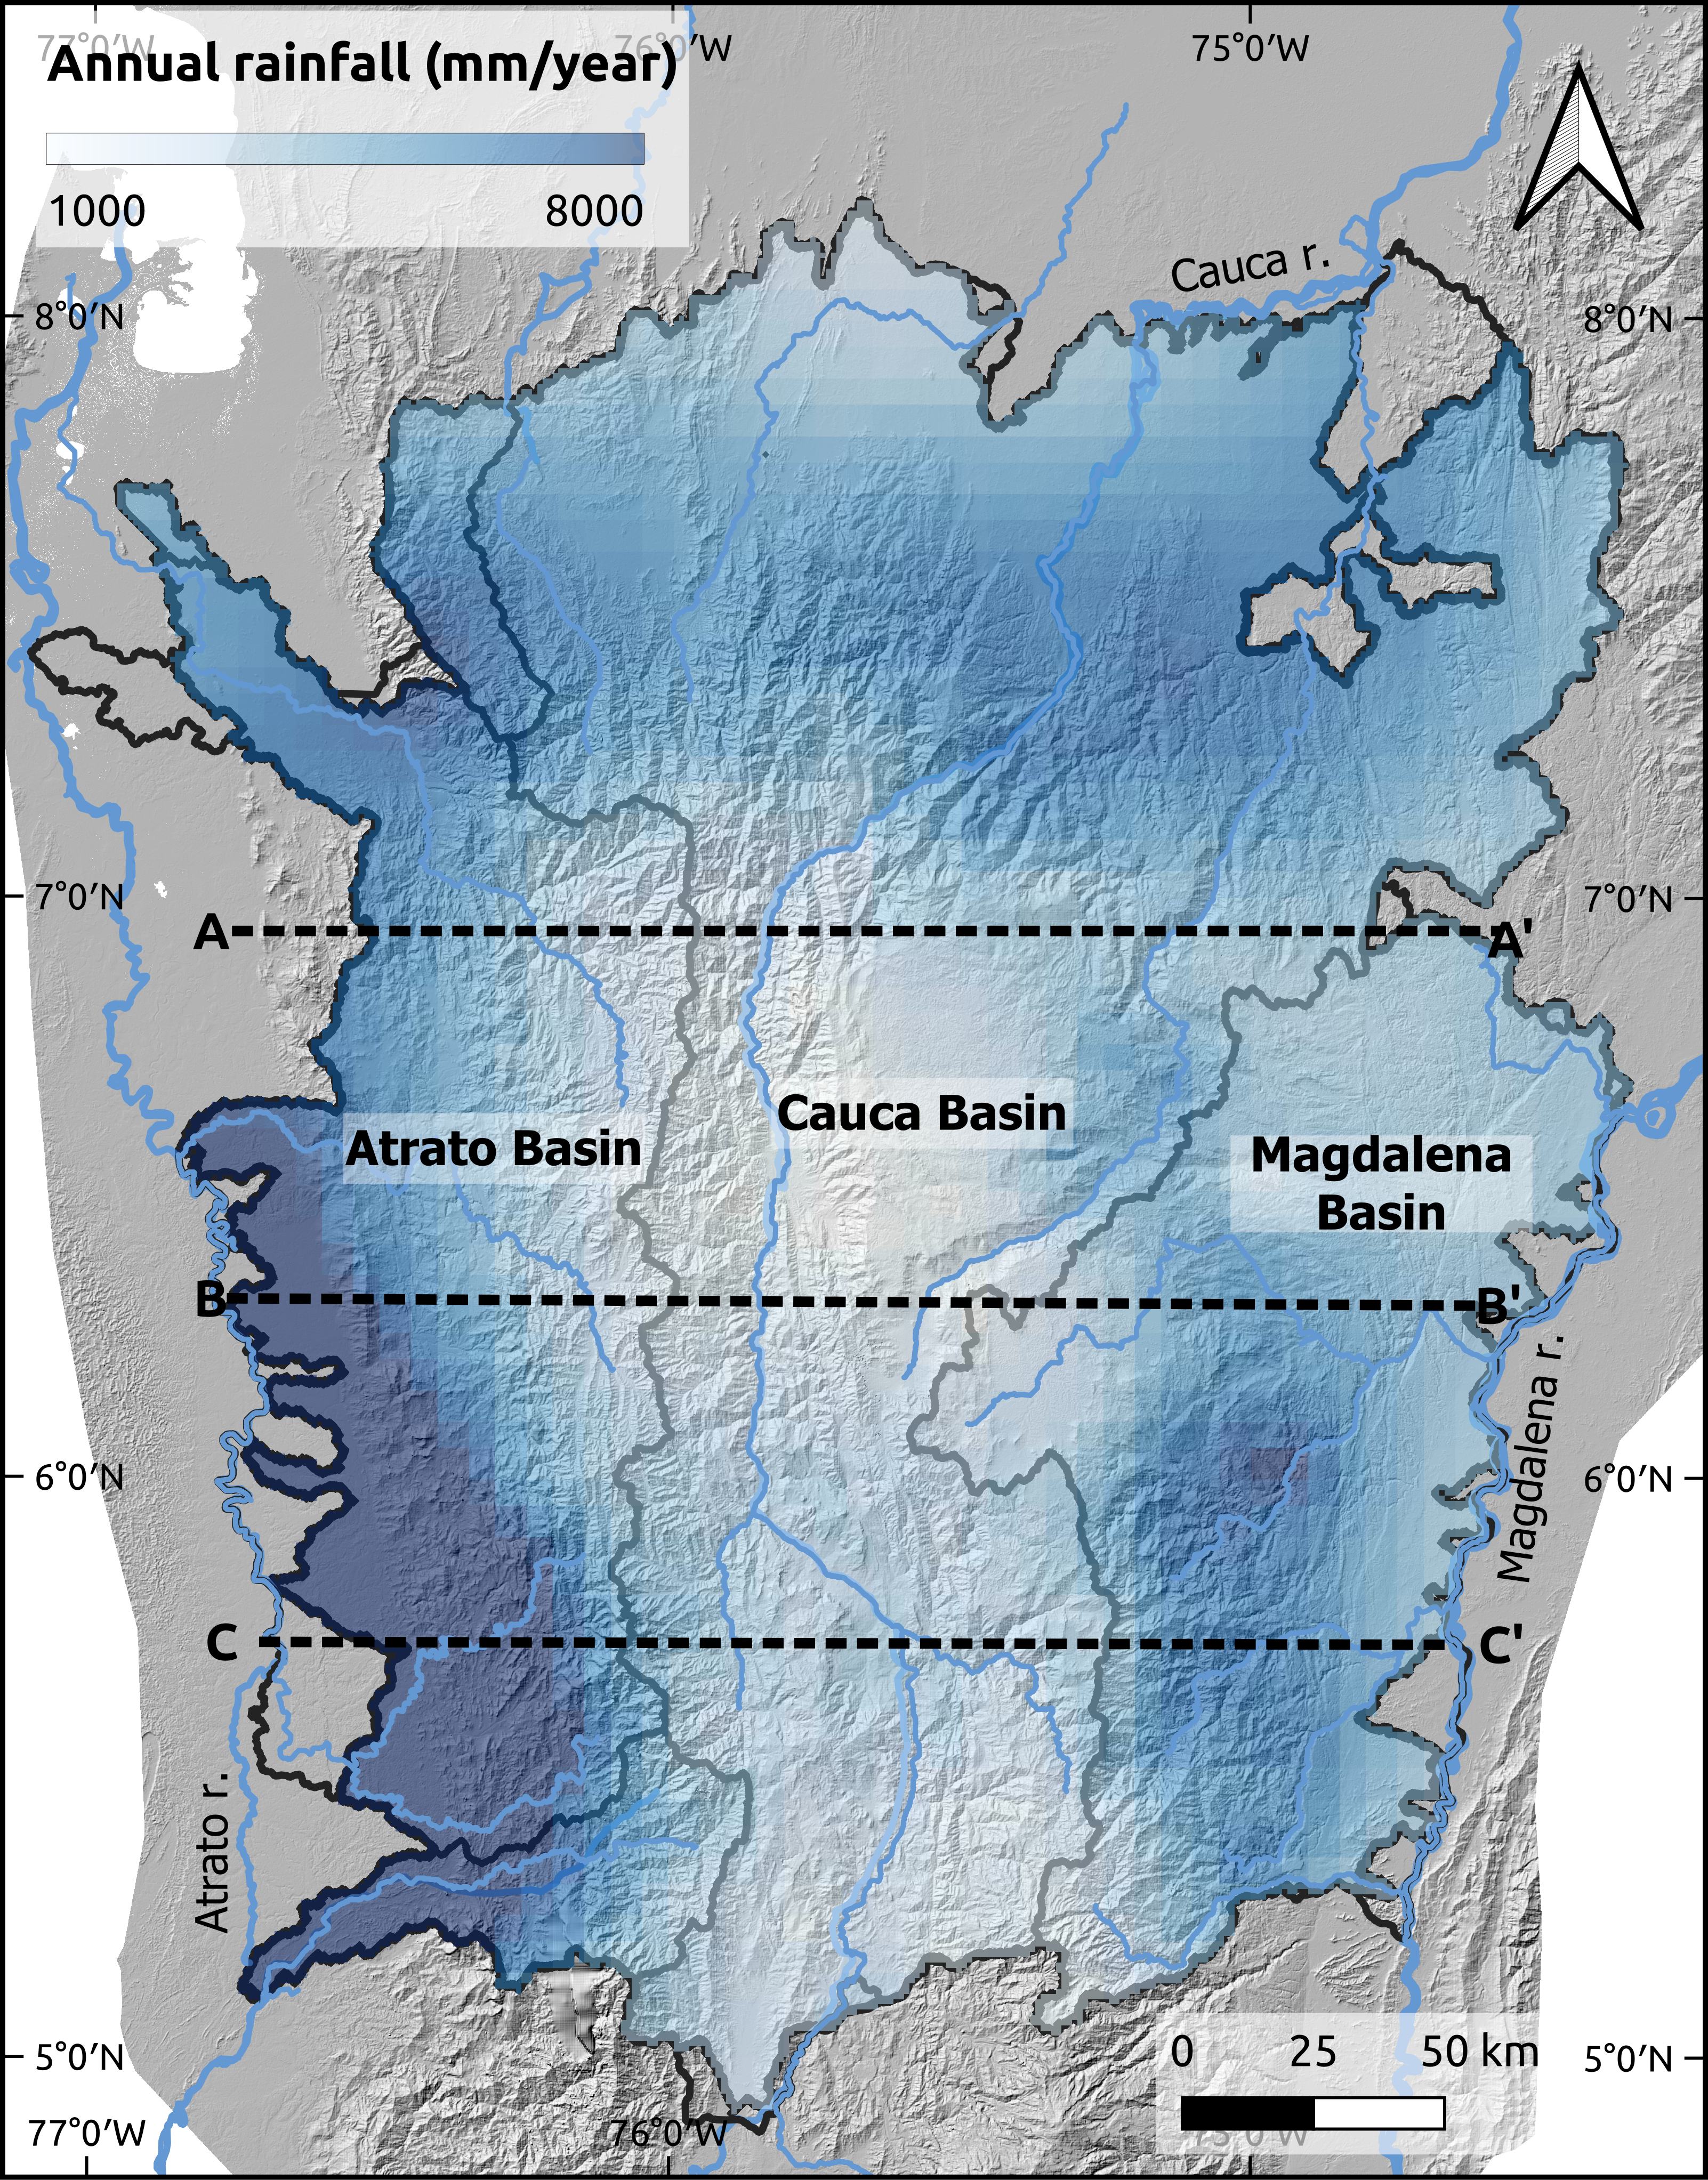
\includegraphics[width=1\textwidth]{rainfall_profile.png}}
  \end{minipage}
  \begin{minipage}{.48\linewidth}
    \centering
      {\includegraphics[width=1\textwidth]{AOI_rainfall_A.png}}
     {\includegraphics[width=1\textwidth]{AOI_rainfall_B.png}}
     {\includegraphics[width=1\textwidth]{AOI_rainfall_C.png}}
   \end{minipage}\quad
    \caption{Mean annual rainfall (1981-2023) from CHIRPS data \cite{funk2015} in the study area. A, B and C are 10-km swath profiles, where black lines are mean elevation and red shades show 1-km local relief; blue bars are mean annual rainfall. The study area covers parts of the Central and Western Cordillera, separated by the Cauca canyon, and bounded by the Atrato and Magdalena rivers in the west and east, respectively.}
    \label{fig:rainfall}
\end{figure}

\par Dense forest covers the WC terrains and the eastern flank of the CC. Whiles, grass covers high lands of the AP and low lands in the north and across the Magdalena valley bottom.

\par The study area is generally considered to be landslide-prone terrain \cite{aristizabal2020spatial, gomez2023spatial}. History of the region has been characterized by numerous occurrences of landslides, some of which have led to significant loss of life and substantial economic impacts. The majority of the landslides initiated along the contact of the residual soil with the saprolite as shallow translational slides, that in many cases are transformed into debris flow due to its high water content. Several of those shallow landslides were identified as landslide clusters across the upper mountains of the CC and WC with dense forest covers. Deep-seated landslides with multiple retrogressive and successive rotational slides are observed along some narrow and low order drainages.

\par Yet, most documented landslides have a strong spatial bias toward urban areas, as historical or media reports tend to focus on landslides causing damage in populated areas \cite{guzzetti2012landslide, froude2018global}. Hence, much information about landslides comes from optical remote sensing, which is compromised by frequent cloud in the northern and western fringes of our study area especially. Rainfall has triggered 92\% of all landslides reported in the Colombian Andes between 1970 and 2023, while strong earthquakes or active volcanism were absent during this period. \cite{aristizabal2020}. The triggers of older landslides generally remain unknown, but strong seismic ground shaking is a likely mechanism for generating even larger slope failures than those reported in the past decades. Many catchments host evidence of large scars and deposits of older landslides that have eluded any systematic documentation so far.

%%%%%%%%%%%%%%%%%%%%%%%%%%%%%%%%%%%%%%%%%%%%%%%%%%%%%%%%%%%%%%%%%

\section{Data and Methods}
\par From the viewpoint of inferring process from form, various morphometric methods, such as hypsometric analysis \cite{Strahler1952} or river longitudinal profiles \cite{Wobus2006}, have been popular to measure topography as the time-integrated result of coupled tectonics, climate, and erosion \cite{Whittaker2012, Perron2013, Willett2014}. Hence, we used two digital elevation models (DEMs) for a terrain analysis of the entire study area, drawing on data from the Shuttle Radar Topography Mission (SRTM) at 30~m \cite{farr2007}, and the Advanced Land Observing Satellite-Phased Array-Type L-Band Synthetic Aperture Radar (ALOS-PALSAR) at 12.5~m \cite{logan2014}. We estimated local relief as the maximum elevation difference in a 1-km radius using the SRTM DEM in Google Earth Engine \cite{moore2011}. 

\par We compiled two catalogues of landslides based on their (un-)known timing: we mapped recent landslides that occurred between 1970 and 2023 (Fig. \ref{fig:inventory}) from high-resolution ($<$1~m) optical satellite images in Google Earth™. Apart from contrasts in color and terrain, we use fresh scars of bare soil as the key diagnostic of landsliding. We separately mapped pre-historic landslides that are mainly deep-seated and that eluded historic landslide databases or optical satellite imagery, but remain well preserved or large enough to stand out in the SRTM and ALOS-PALSAR DEMs. All of these pre-historic landslides have a clearly defined head scarp and body (Fig.~\ref{fig:ripley}A).

\begin{figure}[ht!]
  \begin{minipage}{.48\linewidth}
    \centering
    {\includegraphics[width=1\textwidth]{relict_inv.png}}
   \end{minipage}\quad
   \begin{minipage}{.48\linewidth}
    \centering
      {\includegraphics[width=1\textwidth]{recent_inv.png}}
  \end{minipage}
    \caption{Distribution of 222 pre-historic (with unknown dates, though likely prehistoric) landslides and 13,777 recent landslides (known to have occurred between 1970 and 2023) in the study area. The points mark the centroid of landslide scarps.}
    \label{fig:inventory}
\end{figure}

\par To gauge the influence of the tectonic history on landslide occurrence, we extracted the density of geological lineaments using the LINE algorithms of the image processing and optimization software CATALYST on the SRTM data, based on eight hillshade directions with 45°-bins of azimuth, at a sun elevation of 45°. Given the size of the study area, we only considered lineaments $>$1~km.  

\par We used the Climate Hazard Group InfraRed Precipitation with Station Data (CHIRPS) \cite{funk2015}, version 2.0, to obtain rainfall data at 5-km resolution from 1981 to 2023. 

\par We derived river longitudinal profiles and local slope and elevation data with QGIS. To detect knickpoints, we used TopoToolbox's KnickpointFinder function \cite{Schwanghart_2014}, which iteratively adjusts river profiles to a strictly concave upward shape with a tolerance value that we set to 100~m using the 12.5~m DEM. 

\par We computed the hypsometric integral $H_i$ for the 650 catchments in the study area using WhiteToolBox \cite{lindasy2014} and the ALOS-PALSAR data; $H_i$ is a measure of the "volume" of the catchment bounded by its divides, and has been used as proxy for a stage in landscape development \cite{Strahler1952, Gallen2011}. To identify objectively these stages, we tested several clustering methods to group catchment-wide and binned normalised elevation data into similar classes of basin hypsometry. We considered $K$-means clustering with a Euclidean distance; time series $K$-means with a Dynamic Time Warping (DTW) and a soft DTW metric; and Agglomerative Clustering with a connectivity matrix using different $K$-nearest neighbours for $K$ = 1, 2, 4, and 10. To this end, we used the Python Scikit-Learn library \cite{scikit-learn2011}. We used the elbow method to estimate the optimal number of clusters by plotting the within-cluster sum of squares (WCSS) as a function of $K$ to identify the break point where the rate of decrease in WCSS changes most \cite{thorndike1953}. We also used the Silhouette coefficient (Sc) to measure how similar a catchment is to its own cluster (cohesion) versus other clusters (separation), and ranges from -1 (not clustered) to +1 (clustered) \cite{rousseeuw1987}. 

\par We used the detachment-limited stream-power incision model, which treats erosion rate ($E$) as a power-law function of upstream drainage area ($A$) and local channel slope ($S$) \cite{Howard1983, Whipple1999}, $E=kA^mS^n$, where $m$ and $n$ are empirically derived coefficients as parts of the channel concavity index ($\theta=m/n$), and $k$ is a coefficient that includes the influence of climate, lithology, and other factors \cite{Whipple1999}. Where uplift rate $U$ is balanced by erosion rate ($U=E$), local channel slope can be described as $\partial z/\partial x$=$(U/k)^{1/n}A(x)^{-m/n}$, where $x$ is a channel longitudinal coordinate. \citeA{Perron2013} proposed integrate this equation from a reference point $x_b$:  

\begin{linenomath*}
\begin{equation}
    z(x)= z(x_b)+\left(\frac{U}{KA_0^m}\right)^{1/n}\int_{x_b}^{x} \frac{A_0}{A(x)}^{m/n} \partial{x} \quad \text{or} \quad z(x)=z(x_b)+k_{sn}\chi,
\end{equation}
\end{linenomath*}

where $A_0$ is a reference drainage area to normalize river profiles, and $k_{sn}$ is a local channel steepness metric corrected for upstream drainage area \cite{whipple2017}. This approach transforms the horizontal coordinates of the river profile into a variable $\chi$ that accounts for longitudinal variations in the drainage area \cite{Mudd2014}. \citeA{Willett2014} proposed using $\chi$-maps for interpreting the dynamics and relative stability of drainage divides. Steady-state catchments should have equal $\chi$ values across shared divides, whereas transient states are inferred from differing $\chi$ values, with divides migrating in the direction of larger $\chi$ \cite{Willett2014}. We estimated $\chi$ and $k_{sn}$ using LSDTopoTools \cite{Mudd2014} and TopoToolbox \cite{Schwanghart_2014} using the SRTM dataset.

%%%%%%%%%%%%%%%%%%%%%%%%%%%%%%%%%%%%%%%%%%%%%%%%%%%%%%%%%%%%%%%%%%%

\section{Results}

\par We detected a total of 222 pre-historic landslides and 13,777 recent landslides (Fig. \ref{fig:inventory}) throughout the Cauca canyon, the northern Atrato basin, and the southeastern Magdalena basin. Landslides are most abundant in the Cauca basin, which a density of 0,25 landslides/km$^2$ in 328 catchments, followed by the Atrato basin with 0,22 landslides/km$^2$ in 133 catchments, and finally, the Magdalena basin with 0,18 landslides/km$^2$ in 130 catchments.

\par Fig \ref{fig:profiles} shows the spatial distribution of recent landslides and knickpoints.  Scatter plot show the distribution and distance to outlet of the knickpoints and the recent landslides with marginal relative histograms. For recent landslides elevation corresponds to a central point in the scarp and the distance to outlet corresponds to the nearest drainage, after projecting the scarp point. We found 558 knickpoints ($>$100m) overall, with a density of 0,013 knickpoints/km$^2$ in the Cauca basin and the Magdalena basin, and 0,007 knickpoints/km$^2$ in the Atrato basin. The major knickpoints, in terms of vertical height, are observed along the border between the AP with the Cauca canyon or the Nechi River. Although, the elevation distribution of recent landslides and knickpoints are statistically different, both of them shows a bimodal distribution for elevation. In a similar way, in terms of outlet distance, both distributions are statistically different, but distributions show peaks at distances of 800, 400 and 200 km for both, recent landslides and knickpoints.

\begin{figure}[ht!]
     \centering
        {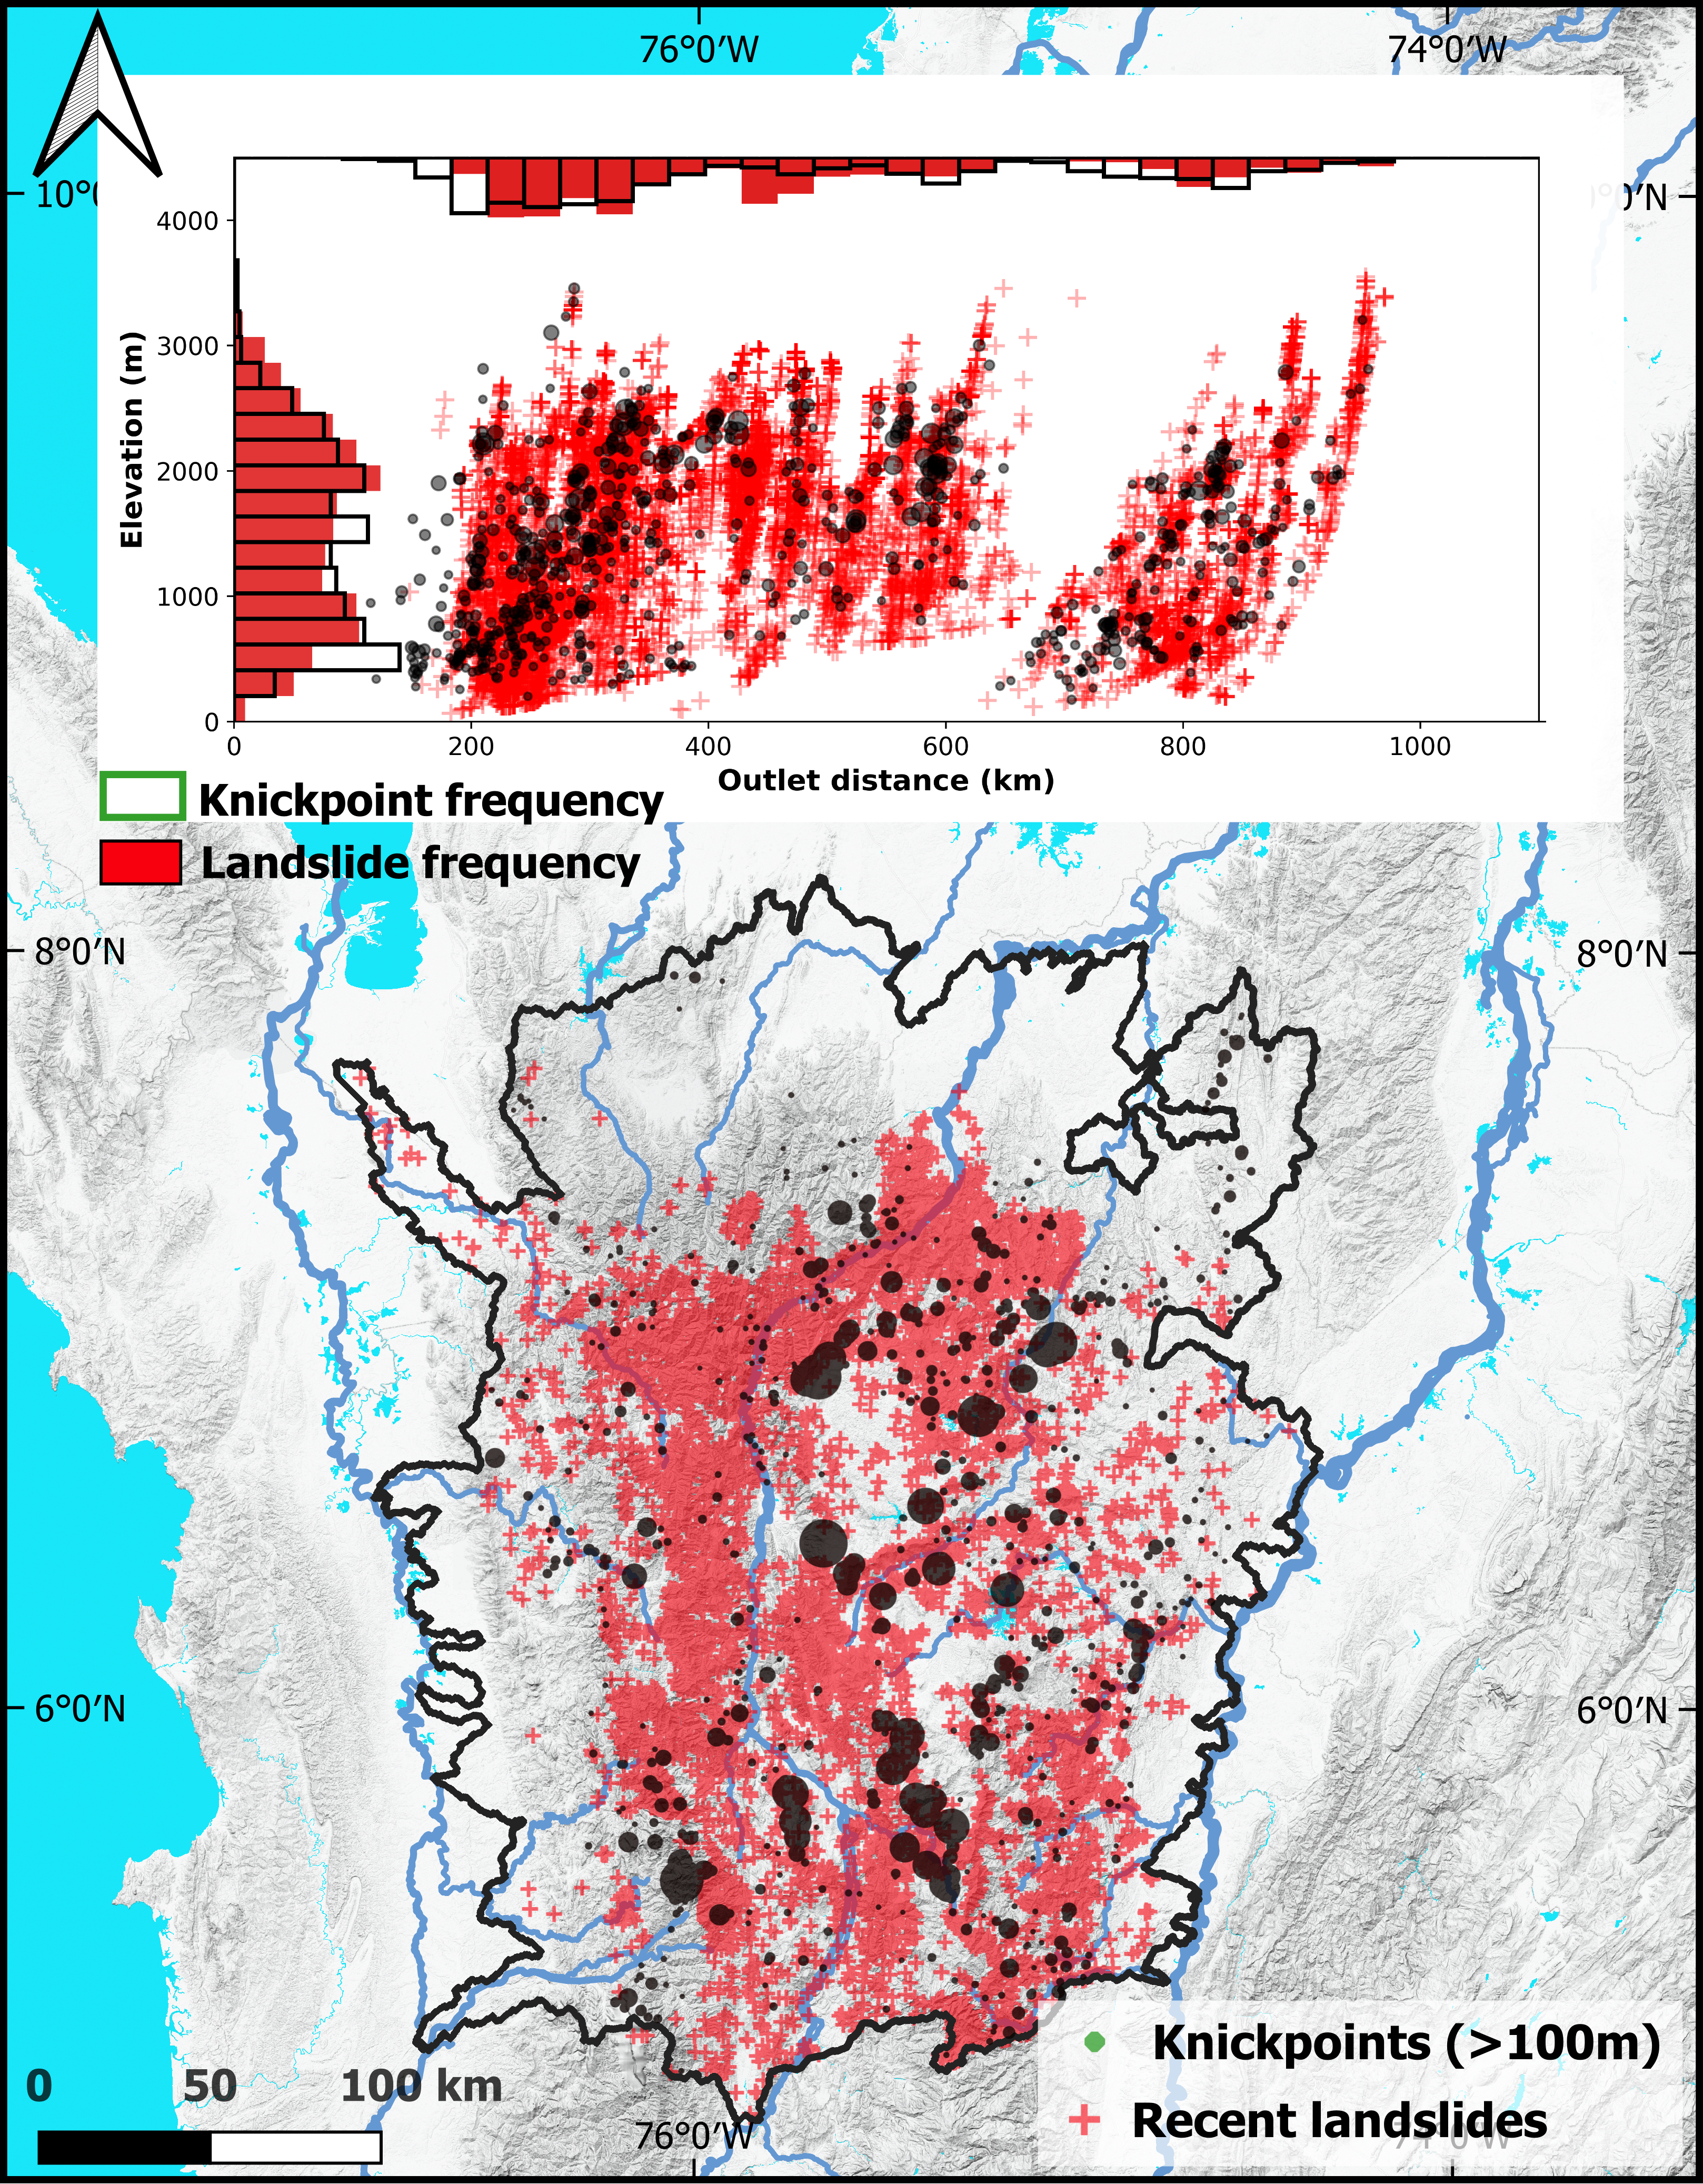
\includegraphics[width=1\textwidth]{river_profile2.png}}
    \caption{Distribution of recent landslides and knickpoints in the study site. Black dots are knickpoints with bubble size scaled to the vertical height of each knickpoint, and red crosses are recent landslides. Marginal histograms show the percentage of recent landslides and knickpoints in terms of elevation and distance from basin outlets. Recent landslides and knickpoints show a similar pattern of elevation and outlet distances.}
  \label{fig:profiles}
\end{figure}

\par Considering there is not a homogeneous landslide distribution for the three basins, and this could be covering different landslide pattern characteristics, we plot landslide distributions with respect to the longitudinal channel network for individual basins ( Fig. \ref{fig:elevationKnickpoints} shows). Both Magdalena and the Atrato Rivers have low gradients of $10^{-4}$ and $10^{-5}$, respectively. The Cauca is the steepest on average ($10^{-3}$), and in contrast with the flatter reaches in the upper Cauca outside of our study area. The three basins show different pattern distributions for recent landslides and knickpoints. In the Magdalena basin prevails landslides and knickpoints in lower elevations. In contrast, in the Atrato basin, recent landslides dominate in higher elevations and knickpoints have bimodal distribution, dominating in the lower and upper basin. For the Cauca basin, both are distributed in the lower and middle basin. In all cases there is observable the coincidence of landslides and knickpoints, except in the Atrato basin, between 200 km and 350 km, where it is observed a clear difference, recent landslides tend to be higher than knickpoints and farther from the basin outlets. 

\begin{figure}[ht!]
    \centering
      {\includegraphics[width=0.8\textwidth]{atrato_landslides.png}}
      {\includegraphics[width=0.8\textwidth]{cauca_landslides.png}}
      {\includegraphics[width=0.8\textwidth]{magdalena_landslides.png}}
    \caption{Distribution of recent landslides (red crosses) (1970 to 2023) and channel knickpoints (black dots). Bubble size scaled to the vertical height of each knickpoint}
    \label{fig:elevationKnickpoints}
\end{figure}

\par Figure \ref{fig:hypso} show $H_i$ for the catchment level. Catchments containing mapped landslides have a distinctly higher $H_i$ than those without (Fig.~\ref{fig:hypso}A). Moreover, catchments containing pre-historic landslides tend to have higher $H_i$ values than those containing recent landslides (Fig. \ref{fig:hypso}A). We find that catchments with landslides have an average local relief of 330~m$\pm$132~m. These catchments have an average slope of 21°$\pm$6°. In contrast, catchments without landslides have an average elevation difference of 185~m$\pm$134~m, and an average slope of 14°$\pm$7°.

\begin{figure}[ht!]
  \begin{minipage}{.48\linewidth}
    \centering
    {\includegraphics[width=1\textwidth]{hypso_rainfall2.png}}
   \end{minipage}\quad
   \begin{minipage}{.48\linewidth}
    \centering
      {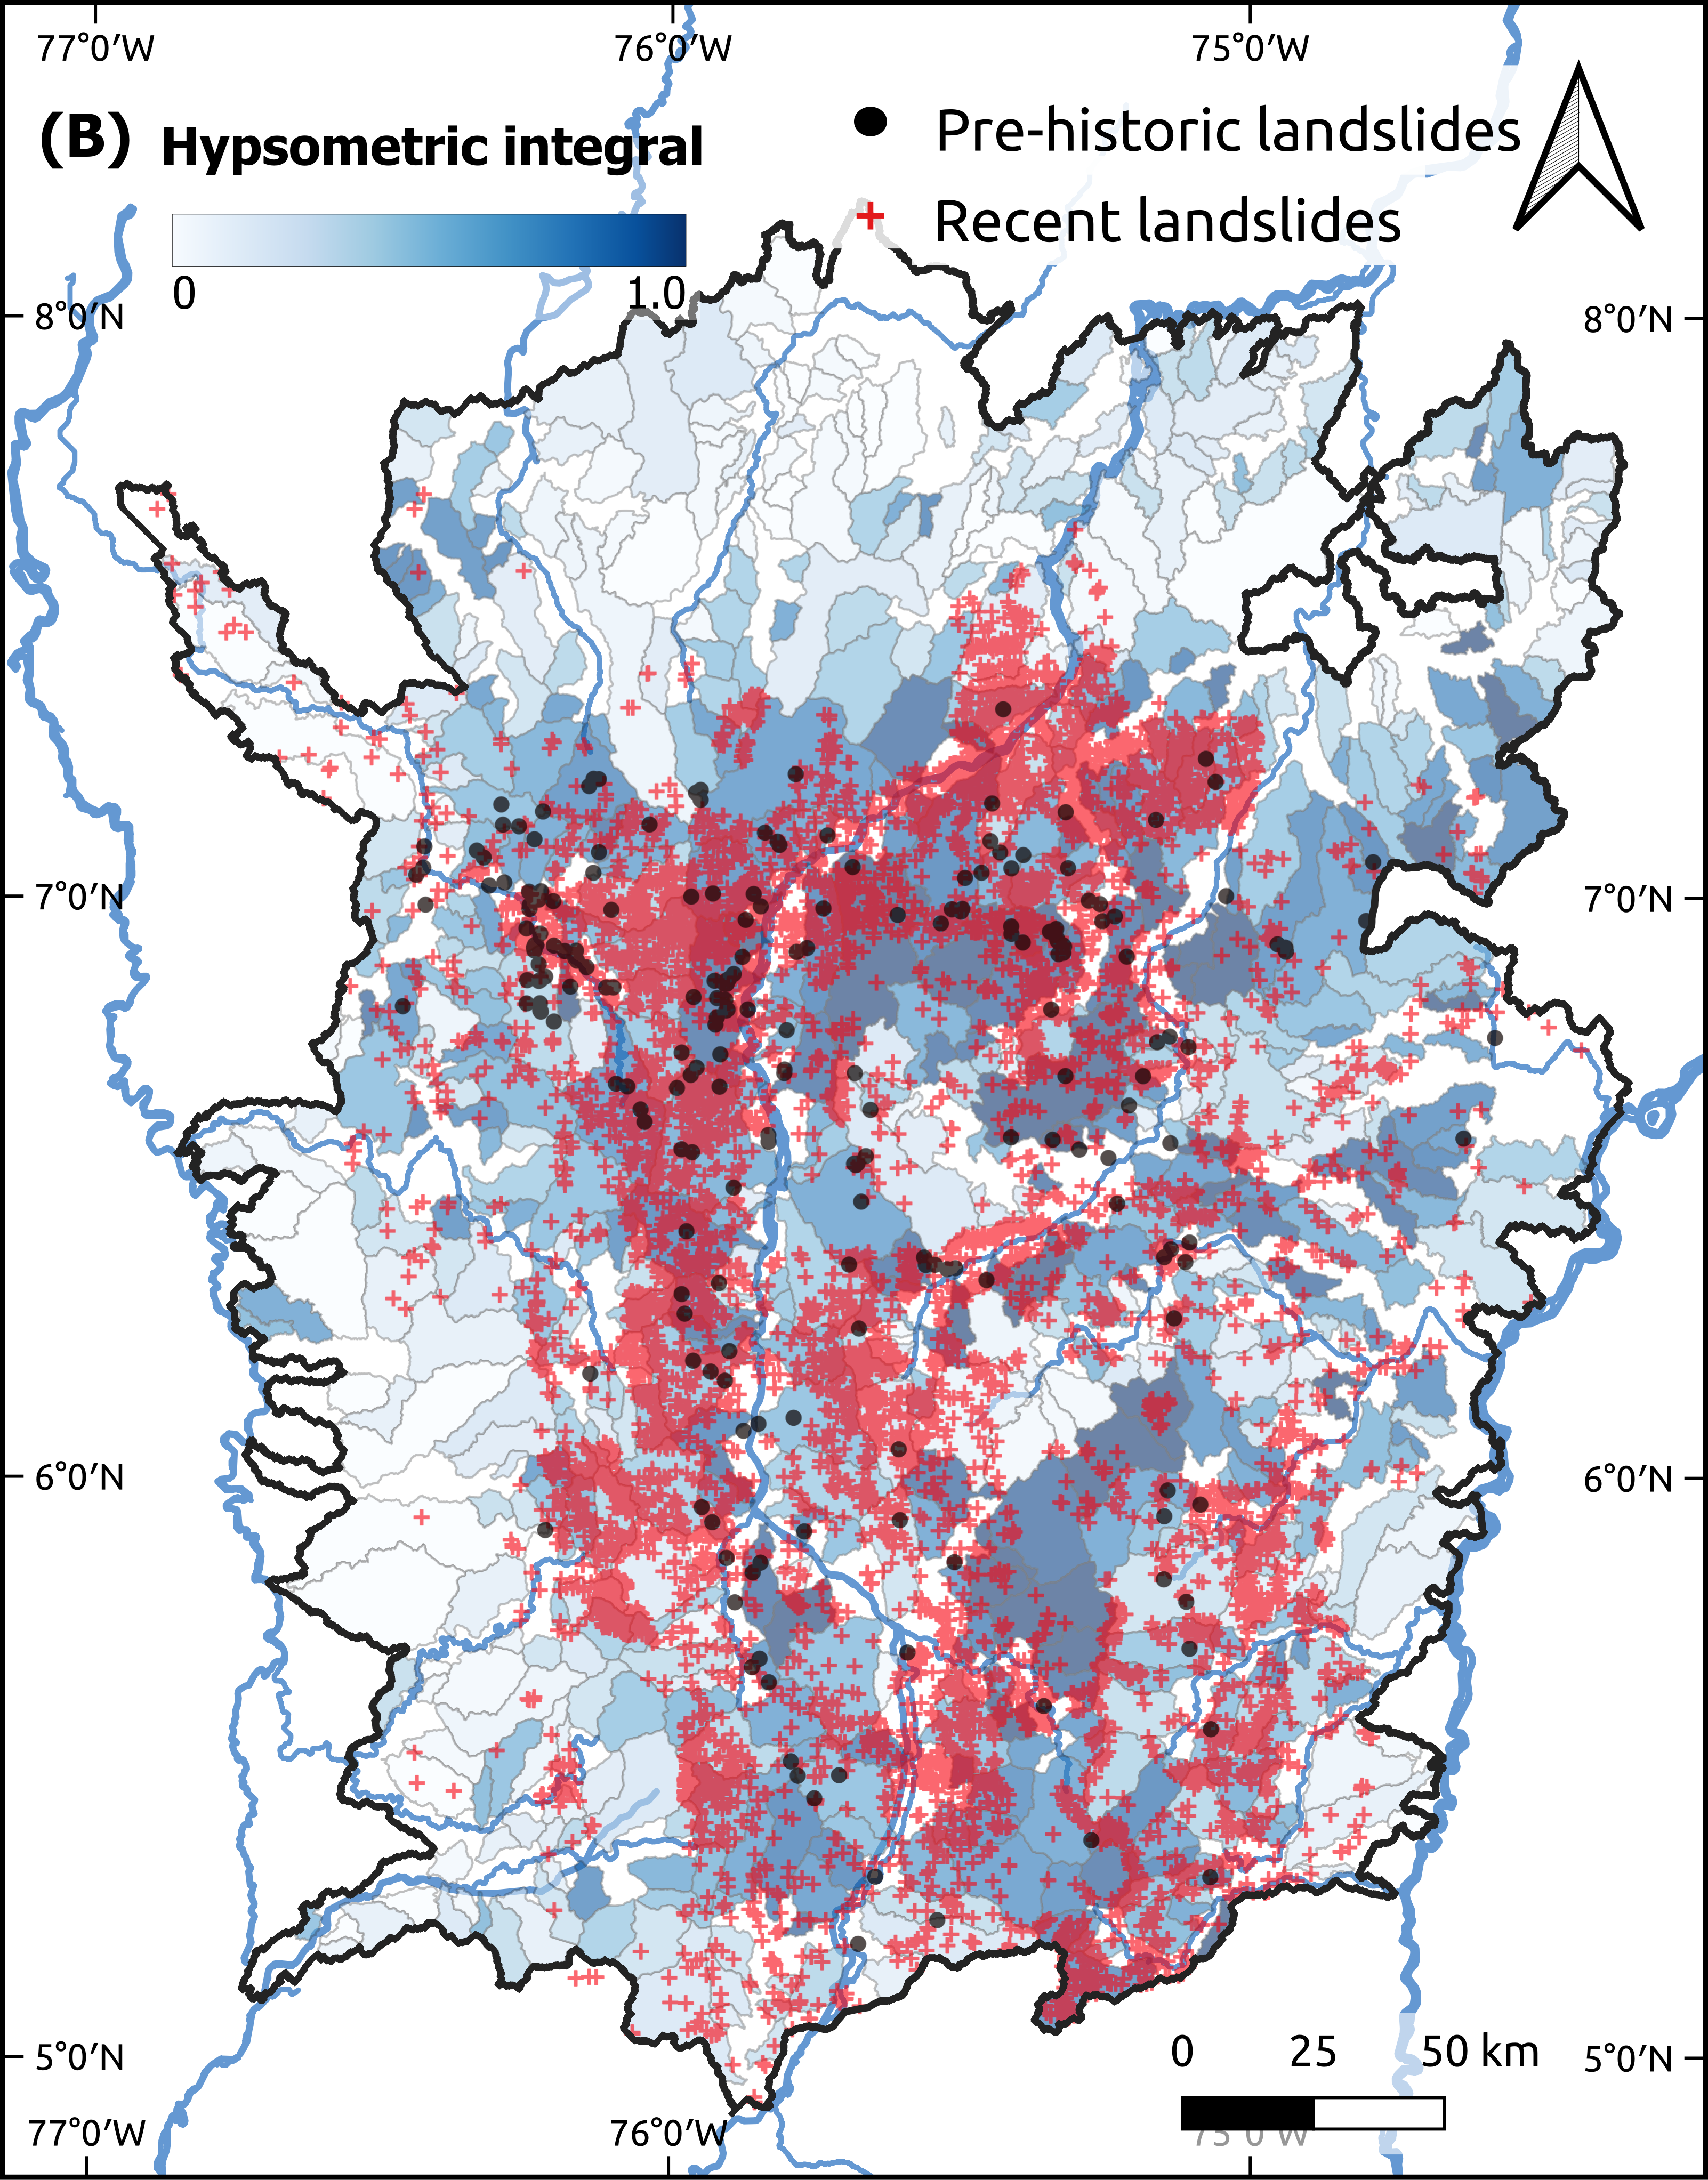
\includegraphics[width=1\textwidth]{hypsometry.png}}
  \end{minipage}
    \caption{(A) Scatter plots of mean annual rainfall versus $H_i$ averaged for each of 650 catchments in the study area (white); catchments with landslides (gray): catchments without landslides (blue); catchments with recent landslides (red): and catchments with pre-historic landslides (black). Bubble size is scaled to the number of landslide in each catchment. Box-and-whisker plots show distributions of $H_i$. (B) Map view of $H_i$.}
    \label{fig:hypso}
\end{figure}

\par The southern region of the study site is characterized by a strong rainfall gradient from west to east, control by the mountain ranges elevations. For the Cauca and Atrato basins, $H_i$ has a negative linear and statistically significant correlation with mean annual rainfall if averaged over catchment area (Fig.~\ref{fig:hypso}A), with coefficients of -1.4 and -6.7, respectively. For more humid catchments such as the Atrato basin the negative gradient is higher. For the Magdalena basin, with mean annual rainfall values much lower compare with the Atrato basin, it shows a slightly positive and not significant correlation. In catchments with recent landslides, their abundance tends to increase with lower $H_i$ and rainfall (Fig.~\ref{fig:hypso}A) with coefficient 0.4. The results from a logistic regression show that the probability that a given catchment has mapped landslides increases with $H_i$ with odds 2.3.

\par Fig.~\ref{fig:knickpoints} shows the results from hypsometric clustering of the 650 catchments. We find that four clusters produced optimal results for the $K$-means algorithm with Euclidean distance and the time series $K$-means algorithm with the softDTW metric. We observe that the hypsometric clusters have distinct peaks at differing normalized elevations. Cluster A has a hypsometric distribution skewed to lower elevations; cluster C has a more symmetric hypsometry, while cluster D is skewed to higher elevations. The spatial arrangement of these clusters is such that cluster A catchments are mainly in the western, eastern, and northern study area, and along the high-elevation, low-relief surfaces of the Cauca and Magdalena basins (Fig.~\ref{fig:knickpoints}A). Cluster B catchments dominate the western flank of the Cauca Canyon, whereas cluster D catchments sit mostly along its eastern flank. Finally, cluster C dominate the western flanks of the northern Cauca River, and its eastern flanks further south. 

\begin{figure}[ht!]
  \begin{minipage}{.68\linewidth}
    \centering
      {\includegraphics[width=1\textwidth]{knickpoint_evolution_Kmeans.png}}
  \end{minipage}\quad
  \begin{minipage}{.28\linewidth}
    \centering
      {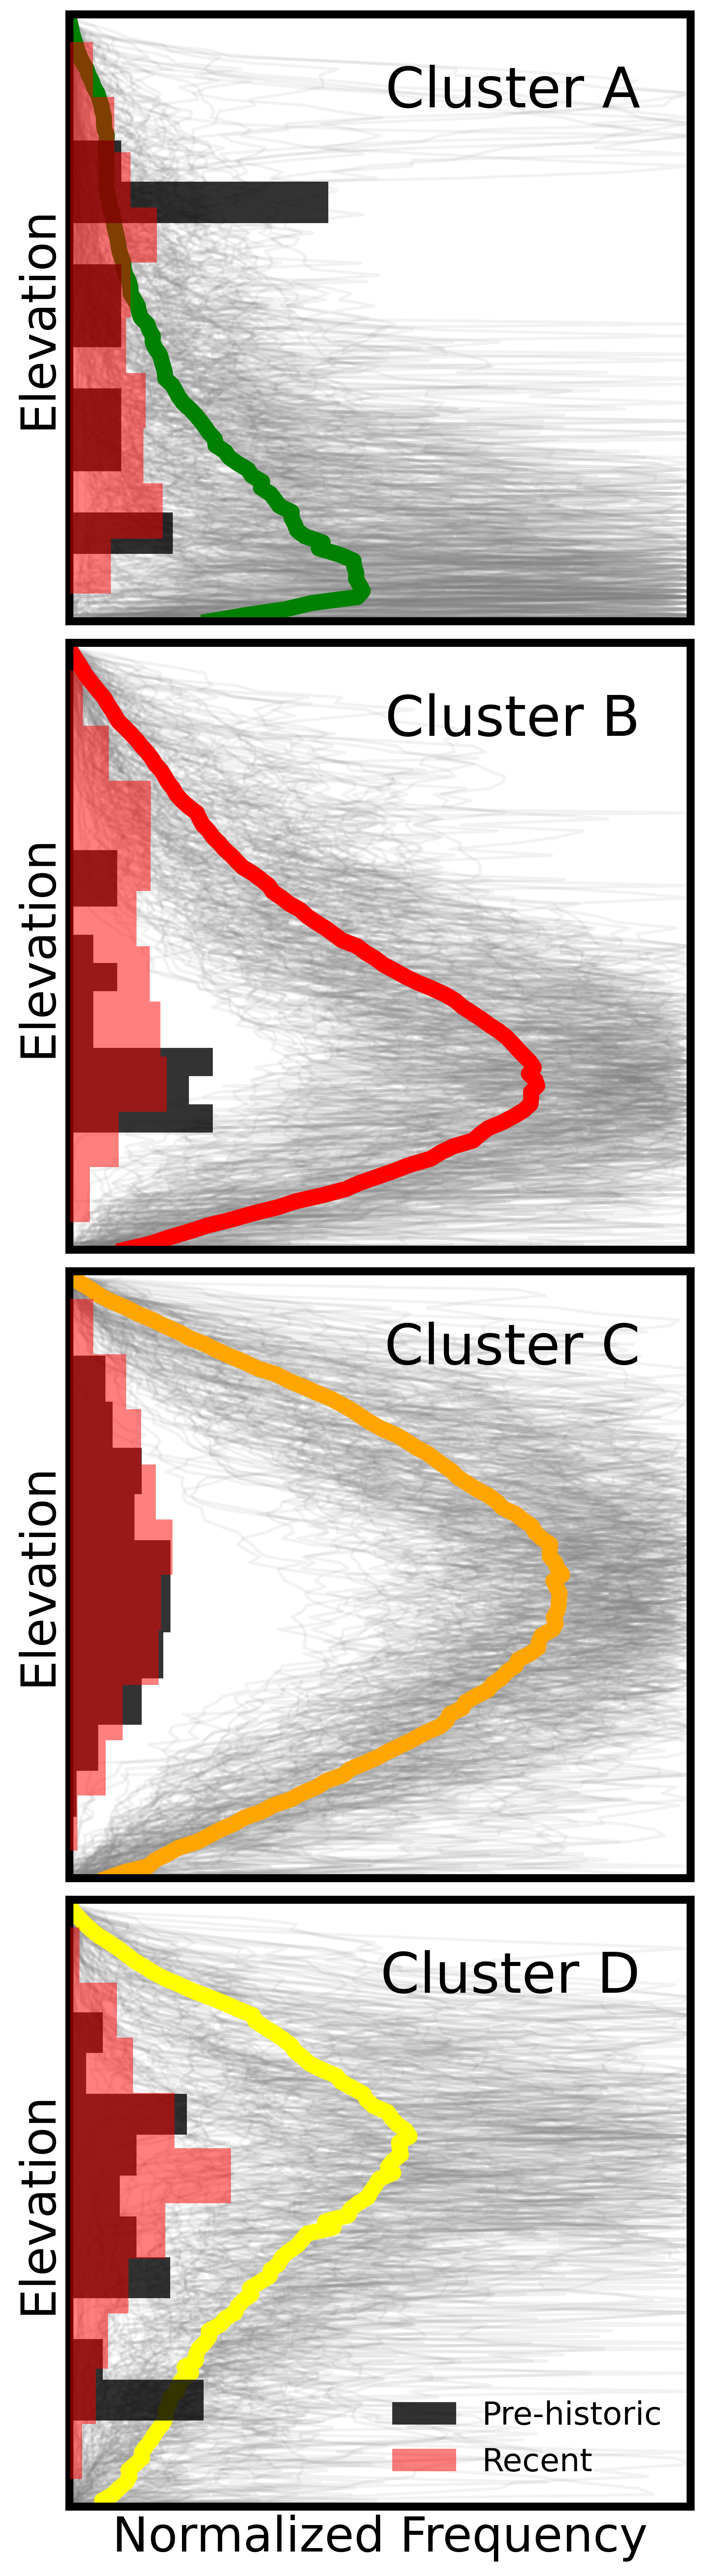
\includegraphics[width=0.8\textwidth] {cluster_knickpoints_kmeans.png}}
  \end{minipage}
    \caption{Cluster analysis of catchment hypsometry reveals four distinct groups (A-D) shown here in map view (left) and as distributions of normalized elevation (color-coded lines, right; grey lines are raw data for each catchment). Clusters A to D identify groups of catchments with shifting dominance from lower to higher relative elevations. Marginal histograms show distribution of recent and pre-historic landslides.}
    \label{fig:knickpoints}
\end{figure}

\par In terms of hypsometric clusters, landslides and knickpoints are concentrated in catchments of Clusters B, C and D. More than half of the pre-historic landslides (53\%) are in catchments of cluster C, followed by clusters D (22\%) and B (16\%). In contrast, 74\% of recent landslides occur in clusters B (36\%) and C (38\%). Knickpoints are mainly distributed in cluster D (39\%) and C (32\%), followed by cluster B (19\%) and A (10\%). The marginal histograms for clusters shows higher distribution of recent landslides close to the elevation peaks, whilst pre-historic landslides in cluster A tends to dominate in higher relative elevations and in Cluster D in relative higher elevations.

\par The clusters have different catchment-wide means of local relief, slope, $H_i$ Integral, and $k_{sn}$ (Fig.~\ref{fig:cluster2}). $H_i$ increases for catchments from cluster A to cluster D.  While mean local relief, mean slope, and mean $k_{sn}$ increase from cluster A to cluster C, and decrease for cluster D (Fig.~\ref{fig:cluster2}).

\begin{figure}[ht!]
     \centering
        {\includegraphics[width=1\textwidth]{cluster_boxplot.png}}
    \caption{Distributions of topographic metrics per hypsometric cluster in Fig.~\ref{fig:knickpoints}. Box-and-whisker plots show medians with notches; whiskers span 1.5~times the interquartile range; bubbles are outside this range. The distributions of each metric differ between the clusters without having been part of the cluster derivation.}
  \label{fig:cluster2}
\end{figure}

\par Fig.~\ref{fig:cluster-profile} shows an example of catchments for each cluster. The plot shows the longitudinal channel profile, hypsometric distribution and landslides. From A to D channel concavity index and $H_i$ increase. Catchments of Cluster A are characterized by channel with high concavities dominated by low relative elevations and low number of landslides with a density of 0.049 landslides/km$^2$. In catchments of Cluster B and C, channel concavity is reduced and landslide density increase to 0.3 landslides/km$^2$. In contrast, catchments of Cluster D tends to have convex channel profiles and landslides slightly decreases (0.218 landslides/km$^2$).

\begin{figure}[ht!]
  \begin{minipage}{.48\linewidth}
    \centering
      {\includegraphics[width=1\textwidth]{rionegro_12m_knickpoints.png}}
      {\includegraphics[width=1\textwidth]{iguana_12m_knickpoints.png}}
  \end{minipage}\quad
  \begin{minipage}{.48\linewidth}
    \centering
      {\includegraphics[width=1\textwidth]{donaMaria_12m_knickpoints.png}}
      {\includegraphics[width=1\textwidth]{garcia_12m_knickpoints.png}}
  \end{minipage}
    \caption{River longitudinal profiles (blue) and hypsometric distributions (marginal histograms) for example catchments from clusters A, B, C and D each. Note the spatial proximity of all four catchments.}
    \label{fig:cluster-profile}
\end{figure}

\par Fig.~\ref{fig:rel-rec} highlights the pattern of $\chi$ for the drainage network, using $A_0=1~\mathrm{km}^2$ and $\theta=0.45$ as proposed by \citeA{Wobus2006}. To compare river profiles in $\chi$ space, we used the confluence of the Cauca and Magdalena Rivers as base level. For the western drainage network, the base level is set by the Atrato River. The number of pre-historic landslides increases with the distance along the first 10~km, whereas the distance of recent landslide from transient divides is constant.

\begin{figure}[ht!]
  \begin{minipage}{.48\linewidth}
    \centering
      {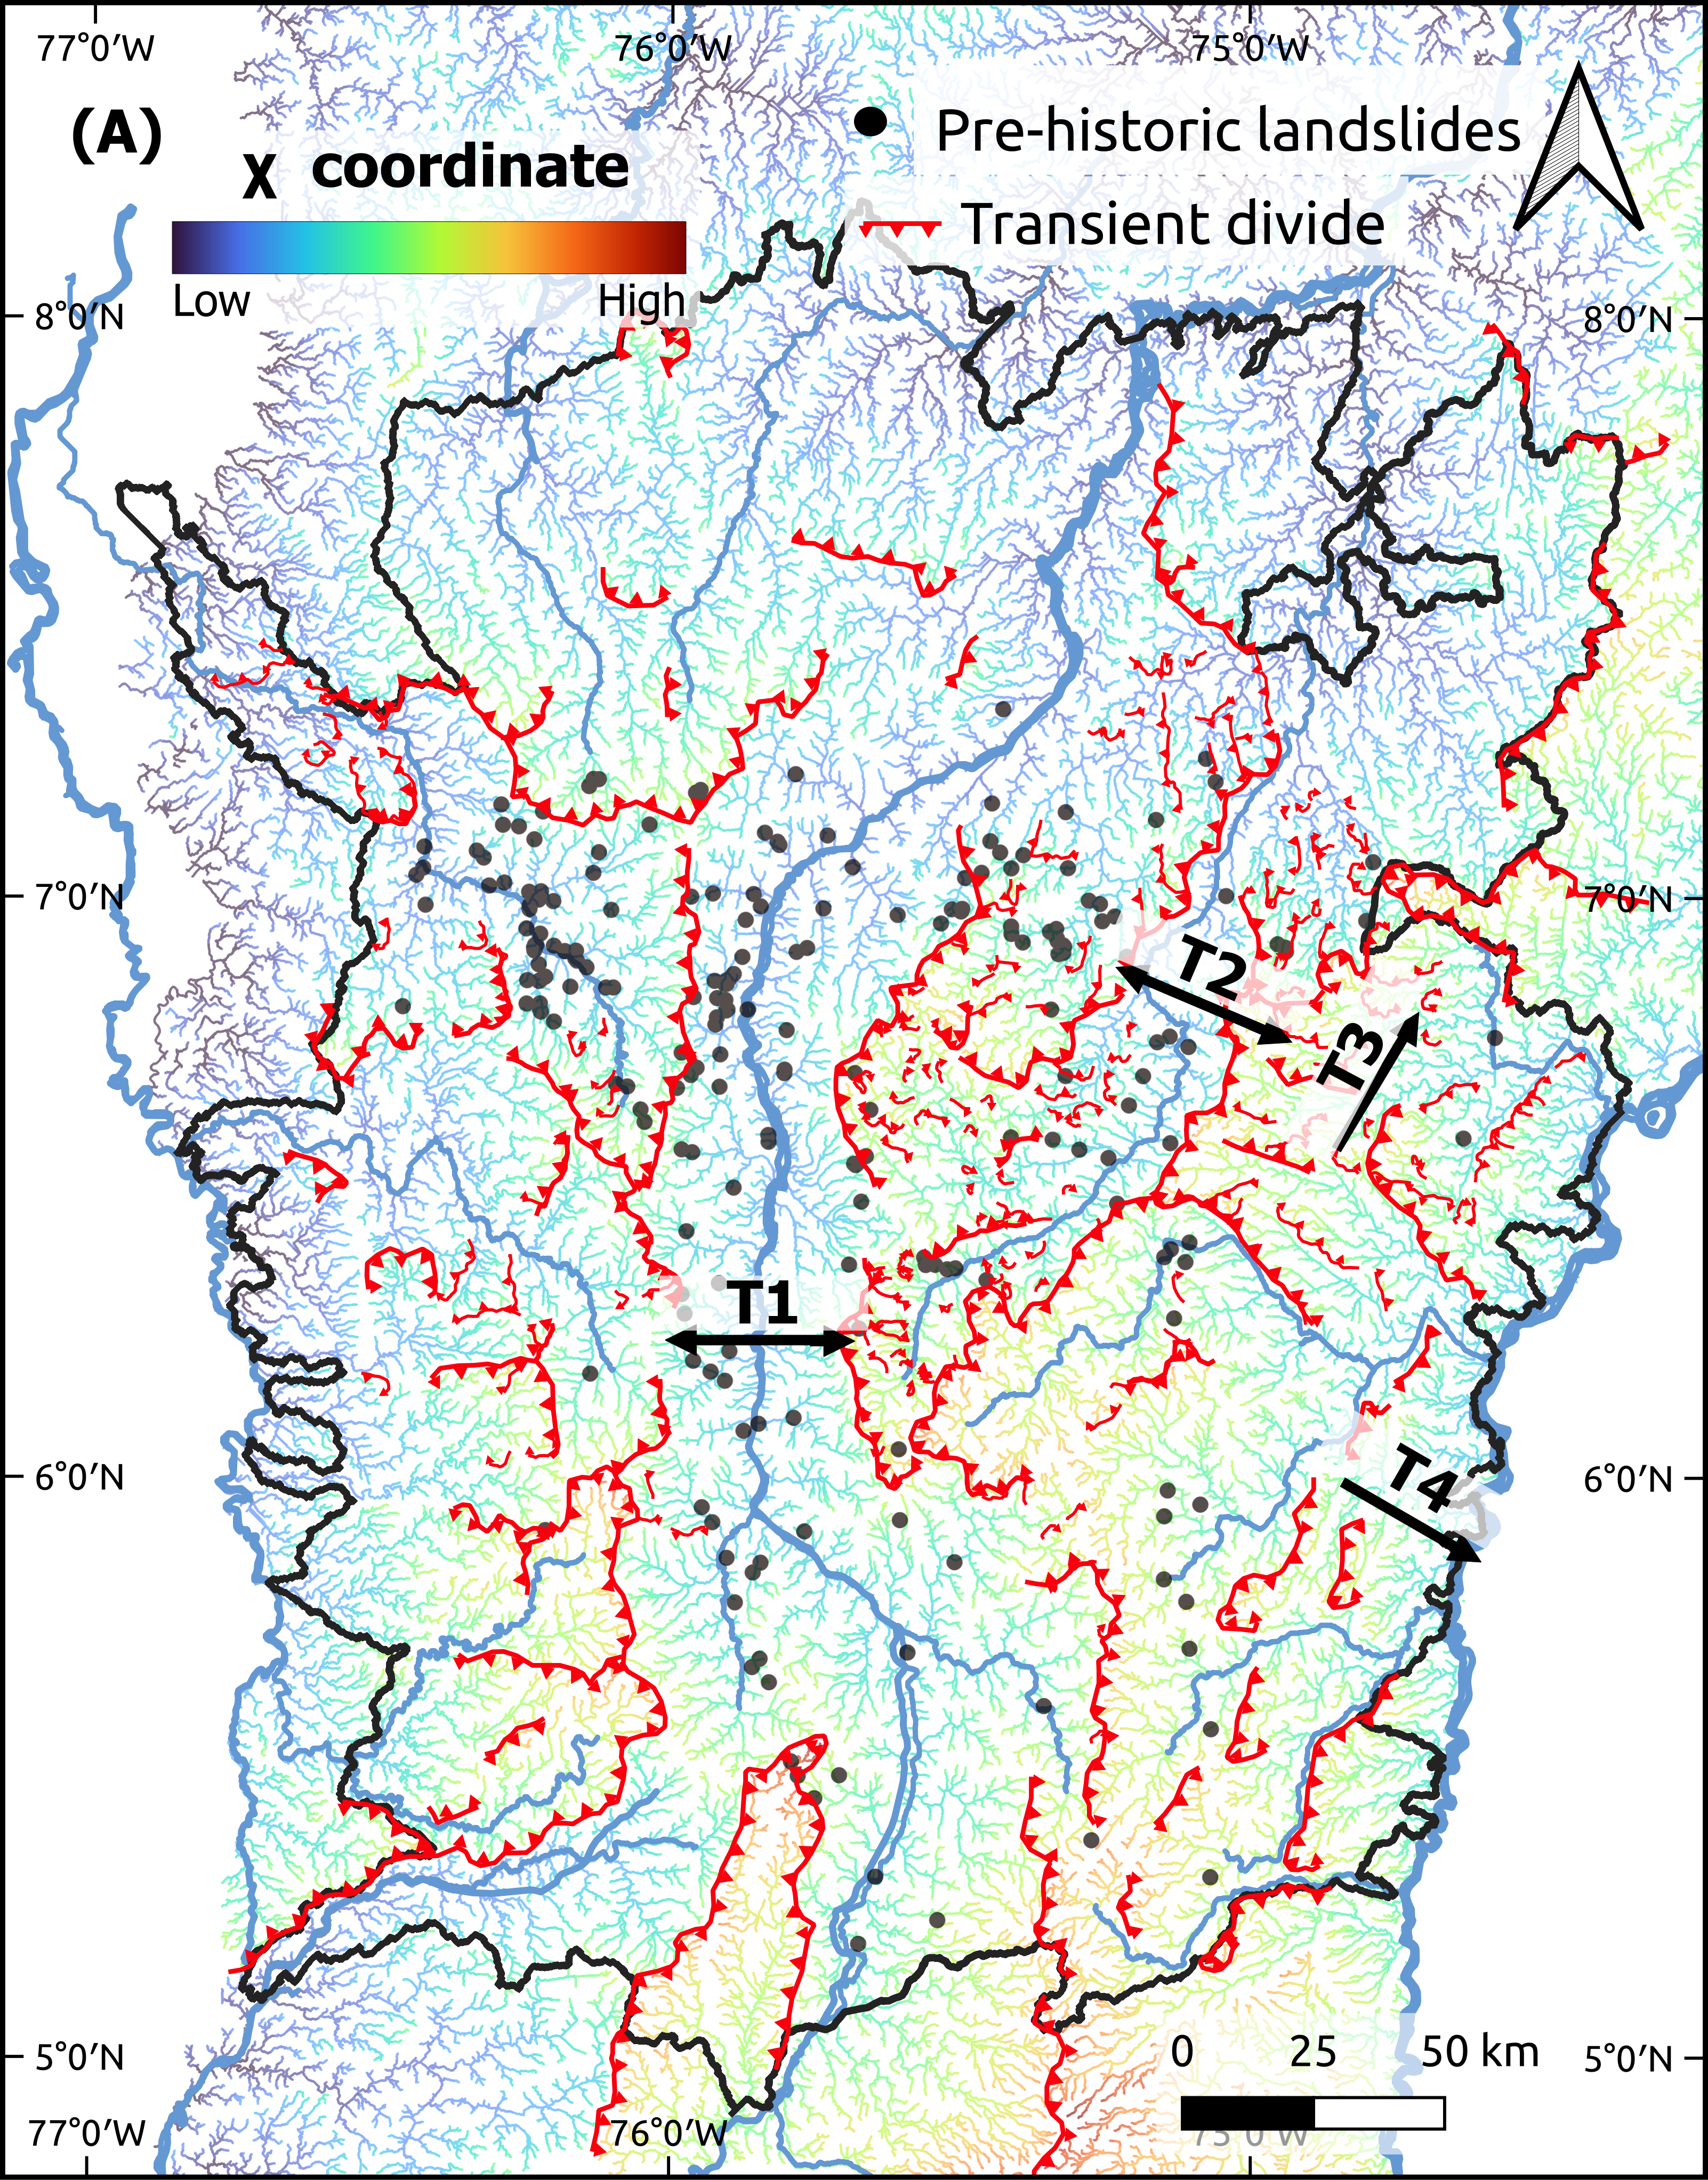
\includegraphics[width=1\textwidth]{border_relicts.png}}
      {\includegraphics[width=1\textwidth]{distance_ancientnorm.png}}
  \end{minipage}\quad
  \begin{minipage}{.48\linewidth}
    \centering
      {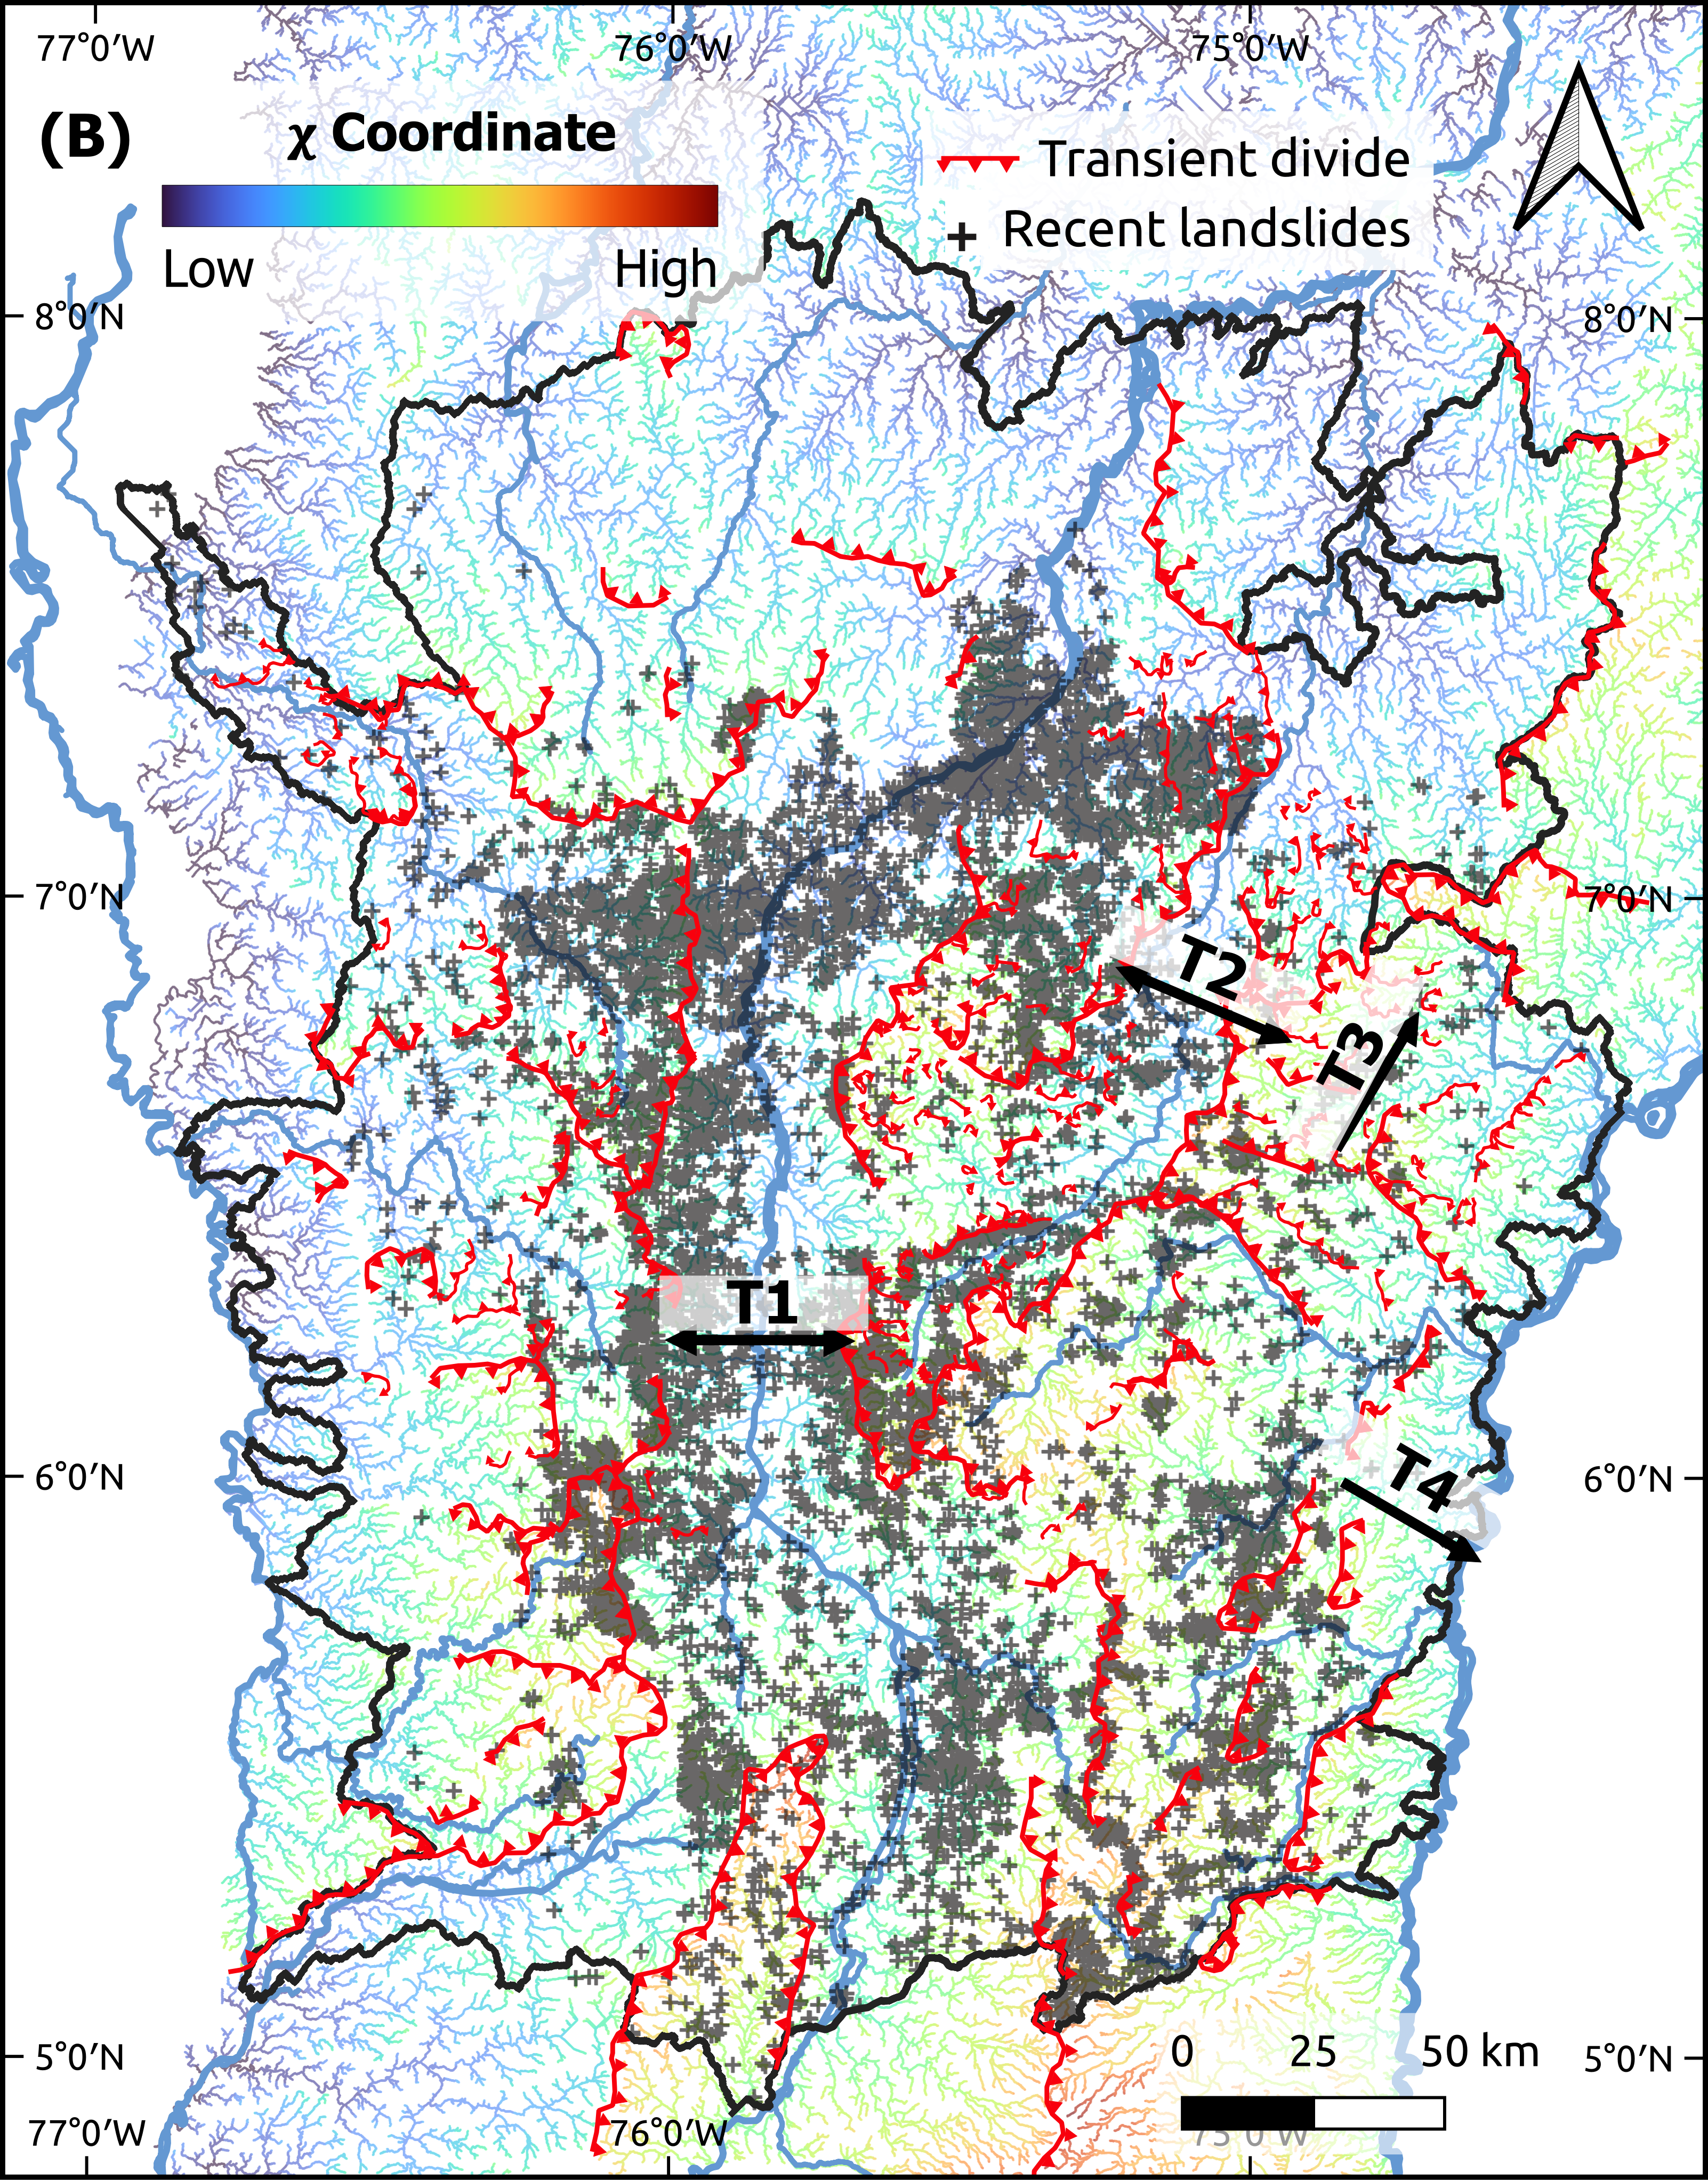
\includegraphics[width=1\textwidth]{border_recients.png}}
      {\includegraphics[width=1\textwidth]{distance_recentnorm.png}}
  \end{minipage}
    \caption{Distribution of $\chi$ along the drainage network of the northern Colombian Andes with pre-historic and recent landslide locations. Red lines are inferred transient drainage divides between main catchments; red arrows indicate the commensurate direction of catchment capture. T1 to T4 mark dominant divide migrating trends. Histograms show distance of landslides from the nearest actively migrating drainage divide in 5-km bins, normalized by fraction of study area at this distance from the divides; a relative frequency of 1 refers to the distance expected for evenly distributed landslides.}
    \label{fig:rel-rec}
\end{figure}

\par We infer competing divides marked by $\chi$ anomalies (Fig.~\ref{fig:rel-rec} dominated by the Cauca River, which captures catchments toward the west and east (T1). The northeastern study area has many transient divides, mainly linked to the Nechi River that undermines catchments to the northwest and southeast (T2). Another divide shifting direction in tributaries of the Nechi is to the northeastern (T3). In the Magdalena basin, divides seem to move to the southeast (T4). The distances from landslide location to transient drainage divides were measured and normalized with no landslide cells.

\par Fig.~\ref{fig:chi} shows pre-historic and recent landslide location with respect to $\chi$. In this plot, channel slope corresponds to $K_{sn}$. Landslides dominate along steep channels which correspond to high erosion rates ($K_{sn}$).

\begin{figure}[ht!]
    \centering
      {\includegraphics[width=1\textwidth]{chi-elevation.png}}
    \caption{$\chi$ plot with pre-historic and recent landslide. Light blue lines correspond to drainage network, and dark blue to the main channels of Atrato, Cauca and Magdalena rivers. $K_{sn}$ corresponds to channel slope.}
    \label{fig:chi}
\end{figure}

%%%%%%%%%%%%%%%%%%%%%%%%%%%%%%%%%%%%%%%%%%

\section{Discussion}

\subsection{Hypsometric clustering}

\par The northern Colombian Andes combine steep mountains and high elevation-low relief terrain in an active tectonic setting. Objective clustering of hypsometric data highlights four distinct groups of catchments with peaks at different relative elevations. Following \cite{Gallen2011}, we interpret these four groups as progressive stages of drainage network development and landscape evolution. We surmise that the variation in catchment mean slope, mean relief, hypsometric distribution, channel concavity and landslide abundance implies that each cluster captures a different stage of landscape evolution (Fig.~\ref{fig:cluster2}). Normalized elevation peaks are lowest in cluster A, and highest in cluster D; Fig.~\ref{fig:knickpoints}A). The distribution of these dominant elevations shifts up in response to tectonic uplift until it fully recovers its state of balanced erosion and re-establishes a predominance of low elevations \cite{Gallen2011}. Catchments in cluster A thus most likely correspond to topographic equilibrium. Increases in uplift rates prompt channels to incise commensurately, thus shifting the hypsometric distribution by increasing the proportion of higher elevations (Cluster B, C, and D), until the channel and hillslopes have adjusted to the new base level (Fig.~\ref{fig:knickpoints}). Steep channels with high values of $K_{sn}$ and contrasting values of $\chi$ across many drainage divides support the idea that catchments with high landslide occurrence are in transient state (Fig.~\ref{fig:rel-rec}).

\subsection{Transient catchments}
\par We associate drainage network metrics with transient state of catchments. Those transient catchments are in areas crossed by numerous geological lineaments and tied to active fault systems (Fig. \ref{fig:structural}). The border of the Cordilleras and the Antioqueño Plateau (AP) dominate the catchments of cluster A. Hypsometric clusters B and C prevail along the western side of the CRFS, thus indicating a disequilibrium, whereas the prevalent cluster D reflect equilibrium along the eastern side (Fig.~\ref{fig:knickpoints}). We interpret this as a consequence of tectonic uplift of the western block or non-uniform uplifting, with higher rates to the west, similar to \citeA{perez2021}, who proposed that increased surface uplift decays eastward. According to the distribution of transient catchments, we propose a decrease towards the northeast. Our results show that southeastern catchments are moving away from a equilibrium state, probably associated to recent activation of the Palestina fault \cite{acosta2007, feininger1970}. This interpretation is consistent with four dominant trends that we identify the inferred migration of transient catchment divides. Two trends are normal to the Cauca canyon (T1) and the Nechi watershed (T2), while two others have a NE direction (T3) and SE (T4) in the eastern flank of the CC. We consider the Cauca trend (T1)  and the trend T2 as the result of a NE-ward tectonic tilting. The trend T2 supports the idea by \citeA{arias1995}, who argued that the Nechi river is capturing the Grande and Aburra rivers that had drained to the Magdalena River earlier, and now drains into the Cauca basin. 

\subsection{Distribution of landslides}

\par We observe that landslides are not randomly distributed. Morphometric analysis shows that landslides in the northern Colombian Andes occur mainly in catchments with high $H_i$, though rarely in the wettest part of the landscape (Fig.~\ref{fig:hypso}). The negative correlation between mean annual rainfall and $H_i$ is strongest in the Atrato basin and means that drier catchments have higher $H_i$ values, with more pre-historic landslides but fewer recent landslides (Fig.~\ref{fig:hypso}). In the Magdalena basin this correlation is weaker and positive. Overall, landslides are preferably concentrated in transient catchments (Figs.~\ref{fig:knickpoints}, \ref{fig:rel-rec}). Both recent and pre-historic landslides are most common in catchments of cluster C, with 38\% and 53\%, respectively. In contrast, catchments of cluster A show the lowest proportion of recent and pre-historic landslides with only 7\%.

\par Transient hillslopes show steep inclinations and high local relief \cite{Whipple1999, matos2016}, and we proposes landslide activity. Figs.~\ref{fig:elevationKnickpoints} and \ref{fig:profiles} show a link between rivers and landslides in the Colombian Andes at the catchment scale (\ref{fig:hypso}), and landsliding is an effective process for hillslopes to adjust river profiles to equilibrium conditions \cite{burbank1996}. Both knickpoints and changes to hypsometric distributions have been linked to temporally imbalanced rates of erosion and tectonic uplift \cite{perez-pena2009}. Our findings are consistent with the model proposed by \citeA{Gallen2011}, and indicate a link between transient catchments and landslides in the northern Colombian Andes. Local base level fall and knickpoint migration in small catchments have been reported in the Cauca basin, and in the Nechi watershed by \citeA{perez2021}, \citeA{aristizabal2008} and \citeA{Noriega2020}. We interpret that the knickpoints are the result of recent tectonic uplift pulses. \citeA{ott2023} proposed an accelerated surface uplift during the past 5~Myr, associated to the collision of the Panamá-Chocó Block (PCB) and resulting flattening of slab subduction.

\par Our analyses show that catchment rejuvenation may influence the spatial pattern of landslides in the northern Colombian Andes. Steady-state river profiles should result in a graded profile with a concave-up curve, while deviations from a concave shape should mark transient states \cite{Whipple1999, Wobus2006}. Numerous knickpoints move upstream, such as in Dona Maria, La Iguana and La Garcia. However, it is important to keep in mind that the catchment response is complex; the response time of the network drainage is significantly longer than the main channel response \cite{Willett2014}, and the time scales of the hillslope response are longer from those of the river channel \cite{fiona2019}. Making in many cases impossible to a given landslide to a specific knickpoint.

\par Additionally to the difference in the the response framework for channels and hillslope drive by tectonic perturbations, climate influences channel and hillslope response, and its coupling. The northern Colombian Andes is an example of not homogeneous tectonic control, but rainfall changes strongly in short distances (km) affecting at catchment scale. There is a contrast between the Atrato basin, with high mean annual rainfall and strong negative correlation with $H_i$, but higher values of landslide density and lower values of knickpoints density; and the Magdalena basin,  with the lowest values of mean annual rainfall and weakly positive correlation with $H_i$, but low density of landslides and high density of knickpoints. 

\par We point out that the density of pre-historic landslides is highest close ($<$10~km) to transient drainage divides. In contrast, the distribution of recent landslides with respect to these divides hardly differs from a random pattern (Fig.~\ref{fig:rel-rec}). This observation could be a cumulative result of multiple retreating knickpoints that maintain unstable hillslopes close to active drainage divides, as headwaters generally also have higher slopes, local relief. However, geomorphic traces of older, and especially small and shallow, landslides may have been removed by weathering and erosion. Hence we expect most recent landslide activity tied to high erosion rates in transient catchments with steep hillslopes. In contrast, we expect that the legacy of pre-historic landslides is preserved better where erosion rates are lower. \citeA{Campforts2020, Campforts2022} model stochastic landsliding and associated sediment dynamics observing that When the uplift rate is higher than the maximum weathering rate, landslides concentrated near ridges with return periods between $10^3$ and $10^4$ years, while landslides closer to the valley network had return periods up to $10^5$ years.

\par Our findings have implications for landslide susceptibility analyses. Although landsliding is a local phenomenon at the hillslope scale, we argue that hillslope-channel coupling influences landslide susceptibility in both the short and long term. Hence, this susceptibility is likely to be a dynamic, rather than the commonly assumed static, condition controlled by the progressive transient stages in the catchment. Our results support the notion that the hypsometric model proposed by \citeA{Gallen2011} can help to evaluate the current and future state of hillslope stability, at least in our study area.  The catchment scale and hillslope scales must be connected in order to fully comprehend the occurrence of landslides. Our results indicates the evolution stage could provide valuable information for landslide susceptibility, and hypsometric distribution is an adequate proxy to evaluate catchment evolution stage. 

\par Previous studies using thermochronology and morphometric analyses has reported an accelerated surface uplifting during the recent geological history in the northern Colombian Andes \cite{restrepo2019, Noriega2020, perez2021, perez2022, ott2023}. Our study provides new evidence based on landslide distribution that the current Andean landscape in the study area has experienced recent pulses of tectonic uplift. The collision of the Panama-Choco Block (PCB) and the beginning of slab flattening, according to thermochronology data, caused a recent surface uplift over the past 6-7 million years, with higher rates or tectonic uflift to the west \cite{perez2021, ott2023}. This has created up to 3 km of relief throughout the Cauca Canyon. A resulting wave of erosion should have moved upstream along the Nechi river and its tributaries, causing transient states and multiple knickpoints. While our observations support the notion of higher recent uplift rates to the west, they also indicated a tilt to the northeast. The differences in the distribution of pre-historic and recent landslides and active transient divides support this idea. Recent landslide occurrence dominates in transient catchments moving away from an equilibrium state. pre-historic landslides dominate in the north, whereas recent landslides in the south, with a landslide distribution with a NW-SE trend. Hillslopes gradually get flatter toward the northeast, and there is a marked trend of river capture to the northeast of the Nechi River, such as the capture of the paleo-Grande and paleo-Aburrá Rivers by the Nechi River. There are more catchments returning to equilibrium state (cluster D) than in Clusters B and C (moving far away of equilibrium state) to the northeast. The catchments along the PFS show a similar trend; transient catchments moving away from a state of equilibrium (clusters B and C) dominate the SW, supporting the idea of a tilt to the northeast. 

%%%%%%%%%%%%%%%%%%%%%%%%%%%%%%%%%%%%%%%%%%%%%%%%%%%%%%%%%%%%%%%
\section{Conclusions}

\par This study contributes to a deeper understanding of landslide susceptibility in active mountain belts, including a long-term and catchment-scale perspective by elucidating the interplay between landscape evolution legacies and local factors. 

\par Geomorphological processes and tectonic uplift have shaped the landscape of the Northern Colombian Andes. The comprehensive analysis conducted in this study sheds light on the possible intricate relationship between landscape evolution and landslide occurrences in the northern Colombian Andes, in the light of key morphometric parameters that characterise the drainage network and hillslopes, and the hypsometry of drainage basins.

\par The distribution of landslides in the study area exhibits a strong link with the regional tectonic setting. The analysis reveals a dynamic landscape evolution process driven by both tectonic uplift and where climate play an important role. Catchments with higher tectonic uplift rates exhibit higher levels of landscape disequilibrium, characterized by steep slopes, high local relief, high $H_i$ and $K_{sn}$ values, and a higher frequency of landslides. Landslides are closely associated with transient catchments, where ongoing base level changes induce hillslope adjustments. Recent landslides tend to occur in catchments experiencing active uplift and rejuvenation, while pre-historic landslides are more prevalent in catchments closer to equilibrium.  

\par Our study emphasizes the importance of catchment rejuvenation and drainage reorganization, in shaping landscape morphology and influencing landslide distribution. Transient catchment divides play a crucial role in transferring landscape perturbations and triggering landslides.  

\par Understanding the interplay between geomorphological processes, landscape evolution, and natural hazards is crucial for sustainable risk management and land-use planning. By analyzing the occurrence of landslides in the northern Colombian Andes, this study provides valuable insights into the complex landscape dynamics and the interaction between hillslopes and channels in response to environmental changes. 

\par The regional catchment and local hillslope scales must be connected in order to fully comprehend the occurrence of past, current and future landslides. While landslides manifest locally, their distribution both spatially and temporally is dominated by regional tectonic or climatic factors. This thorough knowledge would naturally enhance long-term comprehension, which is crucial in the context of global climate and land-use change.

%%%%%%%%%%%%%%%%%%%%%%%%%%%%%%%%
\section{Open Research}
Databases and code used for this study are fully available in Github (https://github.com/edieraristizabal/PAPER_LandscapeEvolutionn).

\acknowledgments
We gratefully acknowledge the support of the Alexander von Humboldt Foundation for awarding the first author with a Georg Forster Research Fellowship for Experienced Researchers. This fellowship has been instrumental in facilitating our research endeavors and has provided invaluable opportunities for collaboration and academic growth.

\bibliography{reference}

\end{document}
